\documentclass[preprint,11pt]{elsarticle}

\usepackage[a4paper,margin=2.5cm]{geometry}
\usepackage{setspace}
\setstretch{1.5}
\usepackage{amsmath,amssymb,amsthm,mathtools}
\usepackage{graphicx}
\usepackage{booktabs}
\usepackage{array}
\usepackage{enumitem}
\usepackage{algorithm}
\usepackage[noend]{algpseudocode}
\usepackage{microtype}
\usepackage[export]{adjustbox}
\usepackage{hyperref}
\hypersetup{hidelinks}
\usepackage{xurl}
\usepackage{orcidlink}
\usepackage{tikz}
\usetikzlibrary{arrows.meta,positioning}

\graphicspath{{../figures/}}
\setlength{\tabcolsep}{4pt}
\renewcommand{\topfraction}{0.9}\renewcommand{\bottomfraction}{0.8}\renewcommand{\textfraction}{0.1}\renewcommand{\floatpagefraction}{0.7}

% ------------------------------------------------------------- theorem environments
\newtheorem{theorem}{Theorem}
\newtheorem{lemma}[theorem]{Lemma}
\newtheorem{proposition}[theorem]{Proposition}
\newtheorem{corollary}[theorem]{Corollary}
\theoremstyle{definition}
\newtheorem{definition}[theorem]{Definition}
\newtheorem{assumption}{Assumption}
\renewcommand{\theassumption}{A\arabic{assumption}}
\newtheorem{example}[theorem]{Example}
\theoremstyle{remark}
\newtheorem{remark}[theorem]{Remark}

% ------------------------------------------------------------- notation
\newcommand{\R}{\mathbb{R}}
\newcommand{\E}{\mathbb{E}}
\newcommand{\cP}{\mathcal{P}}
\newcommand{\cM}{\mathcal{M}}
\newcommand{\cR}{\mathcal{R}}
\newcommand{\ub}{\bar u}
\newcommand{\abar}{\bar a}
\newcommand{\Abar}{\bar A}
\newcommand{\Amax}{A^{\max}}
\newcommand{\conv}{\operatorname{conv}}
\newcommand{\spn}{\operatorname{span}}
\newcommand{\supp}{\operatorname{supp}}
\newcommand{\ICNE}{\mathrm{ICNE}}
\newcommand{\Eu}{\overline{\mathbb{E}}}
\newcommand{\Qb}{\overline{Q}}
\newcommand{\Fl}{\underline{F}}
\newcommand{\Fu}{\overline{F}}
\newcommand{\Pib}{\overline{\Pi}}
\newcommand{\xb}{\bar x}
\newcommand{\pos}[1]{\left(#1\right)^{+}}
\newcommand{\ip}[2]{\langle #1,#2\rangle}
\newcommand{\sd}{\partial^{+}}
\newcommand{\Dl}{\underline{D}}
\newcommand{\Dh}{\overline{D}}

\newcommand{\cQ}{\mathcal{Q}}
\newcommand{\cX}{\mathcal{X}}

% generated by paper/make_tables.py; do not edit
\newcommand{\BRLbetterCities}{Buenos Aires (-1.9\%), New York (-10\%)}
\newcommand{\BRLcgTimeMax}{680}
\newcommand{\BRLcgTimeMin}{13}
\newcommand{\BRLconsMax}{44}
\newcommand{\BRLconsMin}{10}
\newcommand{\BRLequalN}{4}
\newcommand{\BRLfixeduMax}{6.42}
\newcommand{\BRLfixeduN}{20}
\newcommand{\BRLfixeduSub}{9}
\newcommand{\BRLgapMax}{4.0}
\newcommand{\BRLgapMin}{0}
\newcommand{\BRLhdDetTO}{timed out}
\newcommand{\BRLhdN}{25}
\newcommand{\BRLhdScale}{2.5}
\newcommand{\BRLhdTime}{1.8}
\newcommand{\BRLindepMax}{14.1}
\newcommand{\BRLindepMean}{4.5}
\newcommand{\BRLrealCmatch}{18}
\newcommand{\BRLrealCn}{18}
\newcommand{\BRLtestAerr}{$4.5\cdot10^{-14}$}
\newcommand{\BRLtestAn}{40}
\newcommand{\BRLtestCn}{12}
\newcommand{\BRLtimeMax}{0.065}
\newcommand{\BRLtimeMin}{0.004}
\newcommand{\BRLworseCities}{London (+1.3\%), Paris (+0.082\%), Berlin (+0.22\%)}
\newcommand{\CertN}{27}
\newcommand{\CertRegretLPMax}{14}
\newcommand{\CertRegretMax}{$4.5\cdot10^{-13}$}
\newcommand{\EfiveBRasgoodCities}{Cairo, Moscow, New York, Paris, Berlin}
\newcommand{\EfiveBRasgoodN}{5}
\newcommand{\EfiveBRworseCities}{New Delhi, Buenos Aires, Mumbai, London}
\newcommand{\EfiveCallsBRmax}{17}
\newcommand{\EfiveCallsBRmin}{8}
\newcommand{\EfiveCallsCGmax}{143}
\newcommand{\EfiveCallsCGmin}{16}
\newcommand{\EfiveCallsZMCmax}{65}
\newcommand{\EfiveCallsZMCmin}{36}
\newcommand{\EfiveDeffMax}{89}
\newcommand{\EfiveDeffMin}{32}
\newcommand{\EfiveSameN}{6}
\newcommand{\EfiveZMCstrictBestN}{0}
\newcommand{\EfourAllConverged}{all}
\newcommand{\EfourDelta}{0.80}
\newcommand{\EfourEps}{0.41}
\newcommand{\EfourGaDelMax}{100}
\newcommand{\EfourGaDelMin}{31}
\newcommand{\EfourGaWMax}{100}
\newcommand{\EfourGaWMin}{22}
\newcommand{\EfourLondonPb}{-55.7 / -56.2 / -78.2}
\newcommand{\EfourMaxRise}{65}
\newcommand{\EfourMonoCitiesN}{5}
\newcommand{\EfourNonMonoCities}{Moscow, Buenos Aires, Mumbai, Paris}
\newcommand{\EfourNonMonoN}{9}
\newcommand{\EfourPbDelMax}{78}
\newcommand{\EfourPbDelMin}{0}
\newcommand{\EfourPbWMax}{82}
\newcommand{\EfourPbWMin}{2.7}
\newcommand{\EfourRegretMax}{$2.3\cdot10^{-13}$}
\newcommand{\EfourSeeds}{3 seeds}
\newcommand{\EfourSeries}{54}
\newcommand{\EoneCallsMax}{61}
\newcommand{\EoneCallsMin}{40}
\newcommand{\EoneEtaBelowOne}{3}
\newcommand{\EoneEtaMax}{46}
\newcommand{\EoneEtaMin}{0.35}
\newcommand{\EoneHighCities}{Cairo, Moscow, New York, Paris, Berlin}
\newcommand{\EoneLowCities}{New Delhi, Buenos Aires, Mumbai, London}
\newcommand{\EoneRegretLPMax}{19}
\newcommand{\EoneRegretMax}{$2.3\cdot10^{-13}$}
\newcommand{\EoneServedHighMin}{84}
\newcommand{\EoneServedLowMax}{45}
\newcommand{\EoneServedLowMin}{18}
\newcommand{\EoneSlowMax}{17.6}
\newcommand{\EoneSlowMaxCity}{Moscow}
\newcommand{\EoneSlowMin}{0.81}
\newcommand{\EsixBoundMin}{0.875}
\newcommand{\EsixResid}{$3.4\cdot10^{-12}$}
\newcommand{\EthreeSeeds}{3 seeds}
\newcommand{\EtwoBABothMax}{39.7}
\newcommand{\EtwoBABothMin}{28.6}
\newcommand{\EtwoBADelMax}{39.7}
\newcommand{\EtwoBADelMin}{28.6}
\newcommand{\EtwoBothMax}{86.4}
\newcommand{\EtwoBroadBA}{55 / 5.4 / 0}
\newcommand{\EtwoBroadParisServedMax}{8.5}
\newcommand{\EtwoBroadShutdownCities}{New Delhi, Mumbai, London}
\newcommand{\EtwoCongMax}{1.67}
\newcommand{\EtwoCongMaxCase}{Buenos Aires, seed 0}
\newcommand{\EtwoDelhiBothMax}{17.4}
\newcommand{\EtwoDelhiBothMin}{12.2}
\newcommand{\EtwoDelhiDelMax}{16.9}
\newcommand{\EtwoDelhiDelMin}{6.99}
\newcommand{\EtwoDelivSubsidyMaterial}{18 of 18}
\newcommand{\EtwoLondonBothMax}{86.4}
\newcommand{\EtwoLondonBothMin}{34.5}
\newcommand{\EtwoLondonDelMax}{65.6}
\newcommand{\EtwoLondonDelMin}{30.8}
\newcommand{\EtwoMaterialN}{18}
\newcommand{\EtwoMumbaiShares}{0.042 / 0.98 / 0.79}
\newcommand{\EtwoSeeds}{3 seeds}
\newcommand{\EtwoShareGeHalfN}{17}
\newcommand{\EtwoShareLowCases}{Mumbai seed 0 (0.042)}
\newcommand{\EtwoShareRanges}{New Delhi 0.57--0.97, Buenos Aires 1.0--1.0, Mumbai 0.042--0.98, London 0.76--0.89, Paris 0.90--0.99, Berlin 0.79--1.0}
\newcommand{\EtwoSmallCities}{Cairo, Moscow, New York}
\newcommand{\EtwoSmallMax}{0.47}
\newcommand{\EtwoSubsidyMaterial}{18 of 18}
\newcommand{\NCases}{27}
\newcommand{\NCities}{9}
\newcommand{\NEmax}{6}
\newcommand{\NEmin}{2}
\newcommand{\NSeeds}{3}
\newcommand{\PoABAMax}{1.42}
\newcommand{\PoABAMin}{1.31}
\newcommand{\PoADelhiMax}{1.23}
\newcommand{\PoADelhiMin}{1.15}
\newcommand{\PoALondonMax}{1.94}
\newcommand{\PoALondonMin}{1.45}
\newcommand{\PoAhighCities}{New Delhi, Buenos Aires, London}
\newcommand{\PoAlowCities}{Cairo, Moscow, New York, Mumbai, Paris, Berlin}
\newcommand{\PoAlowMax}{1.05}
\newcommand{\PoAlowN}{6}
\newcommand{\PoAmax}{1.94}
\newcommand{\PoAmaxCity}{London}
\newcommand{\PoApricedMax}{1.08}
\newcommand{\PoAworstMax}{1.98}
\newcommand{\PoSgapCases}{Mumbai seed 0 (PoS 1.02, worst 1.11), Buenos Aires seed 1 (PoS 1.41, worst 1.54), London seed 0 (PoS 1.52, worst 1.61), London seed 1 (PoS 1.42, worst 1.67)}
\newcommand{\PoSgapN}{4}
\newcommand{\PoSgapTotal}{27}
\newcommand{\PricedGapDelhiMax}{4.9}
\newcommand{\PricedGapDelhiSeed}{1}
\newcommand{\PricedGapMax}{7.4}
\newcommand{\PricedGapMaxCase}{London, seed 1}
\newcommand{\PricedSmallCities}{Cairo, Moscow, New York, Mumbai, Paris, Berlin}
\newcommand{\PricedSmallN}{6}
\newcommand{\SObound}{25}
\newcommand{\SOboundCity}{London}
\newcommand{\TinyBRglobal}{35}
\newcommand{\TinyCGglobal}{39}
\newcommand{\TinyFWglobal}{38}
\newcommand{\TinyN}{40}
\newcommand{\TinyZMCglobal}{40}
\newcommand{\ZMCsynthN}{20}
\newcommand{\ZMCsynthWins}{17}
\newcommand{\Zmax}{593}
\newcommand{\Zmin}{42}


\newcommand{\SM}[1]{Supplementary Material, Section~#1}
\newcommand{\SMs}[1]{Supplementary Material, Sections~#1}

\begin{document}

% Template-dependent block: title, author, abstract, keywords.
% Everything below is the only part that needs to change when the manuscript is moved to another journal template.
\begin{frontmatter}

\title{City charges for competing delivery carriers: exact best responses under probability-box travel times and leader pricing without equilibrium search}

\author{Quang-Vinh Dang\,\orcidlink{0000-0002-3877-8024}}
\ead{vinh.dq4@buv.edu.vn}
\address{British University Vietnam, Hung Yen, Vietnam}

\begin{abstract}
A city that charges delivery carriers faces a bilevel problem with three stacked difficulties. Each carrier solves an NP-hard routing problem under probability-box travel times with unknown dependence; the carriers play a Cournot-type congestion game; and the usual search over charges solves one equilibrium per grid point, about two thousand routing solves per city. We give three algorithms. Budget-resource labelling prices routes exactly, and branch-and-price makes each carrier's integer plan exact. Its advantage is proof speed and label counts at about 25 customers; it does not beat sample-average plans out of sample and does not scale beyond about 40 customers. Dual implementation pricing makes a social target an equilibrium by best-response cuts. Aggregate-response pricing sets charges from observed zone totals and contracts at a rate independent of instance size. On nine metropolitan areas built from OpenStreetMap and gridded population, with ten seeds in three cities, dual implementation pricing reached \TenDipGridBuenosAires--\TenDipGridNewDelhi{} times the best grid point's gain with \TenDipCallsNewDelhi--\TenDipCallsLondon\% of its calls, and \TenSoDipNewDelhi--\TenSoDipLondon{} of the social optimum's gain (grid: \TenSoGridNewDelhi--\TenSoGridBuenosAires); aggregate-response pricing reached \TenSoArpNewDelhi--\TenSoArpBuenosAires. Pure equilibria exist under exposure-based congestion, and deciding their existence is strongly NP-complete under vehicle-count congestion; the belief-width result is close to earlier work on approximate equilibria. Levels of the price of anarchy, service and gains depend on the criterion the carriers use: with sample-average carriers service roughly doubles. Orderings and policy directions are robust.
\end{abstract}

\begin{keyword}
bilevel optimization \sep vehicle routing \sep imprecise probabilities \sep congestion games \sep branch-and-price \sep road pricing
\end{keyword}

\end{frontmatter}


%======================================================================
\section{Introduction}\label{sec:intro}

Several delivery firms serve the same neighbourhoods, sell to overlapping customers and slow one another down on the same streets. Cities respond with instruments that act on all of them: congestion and low-emission zones, kerbside rules, and charges or subsidies per delivery \citep{Quak2009,HolguinVeras2016,Dey2019,XuSun2024}. As traffic and parcel data become more widely available, the practical question is how to turn such data into charges whose effect can be predicted. Predicting it means predicting how the carriers react, and the reaction is itself the outcome of routing decisions that are hard to compute and rest on noisy travel-time data.

We treat the city as the leader of a bilevel problem with three stacked difficulties.
\begin{enumerate}[label=(\arabic*),leftmargin=*,itemsep=0pt]
\item \emph{Each follower solves an NP-hard routing problem under imprecise probabilities.} A carrier has a few weeks of travel-time observations. These bound the distribution function of each arc time (a probability box) and say nothing about the dependence between arcs. The robust cost of a route is its worst-case expected loss over all joint laws compatible with the boxes.
\item \emph{The followers play a congestion game.} The price a carrier obtains falls with the total deliveries in a zone (Cournot competition) and travel times rise with vehicle density. If congestion depends on vehicle-hours (exposure), the game has an exact potential and pure equilibria exist. If it depends on vehicle counts, deciding whether a pure equilibrium exists is strongly NP-complete (Section~\ref{sec:theory}).
\item \emph{The leader's problem is a bilevel program whose lower level is the game above.} The usual approach evaluates a grid of charges and computes one equilibrium per grid point. With 63 grid points this took \GridCallsFullMin--\GridCallsFullMax{} routing-oracle calls per city and seed in our experiments, each call an NP-hard problem.
\end{enumerate}
We give an algorithm for each layer (Figure~\ref{fig:layers}) and test them on nine metropolitan areas.

\begin{figure}[tbp]\centering
\resizebox{\textwidth}{!}{%
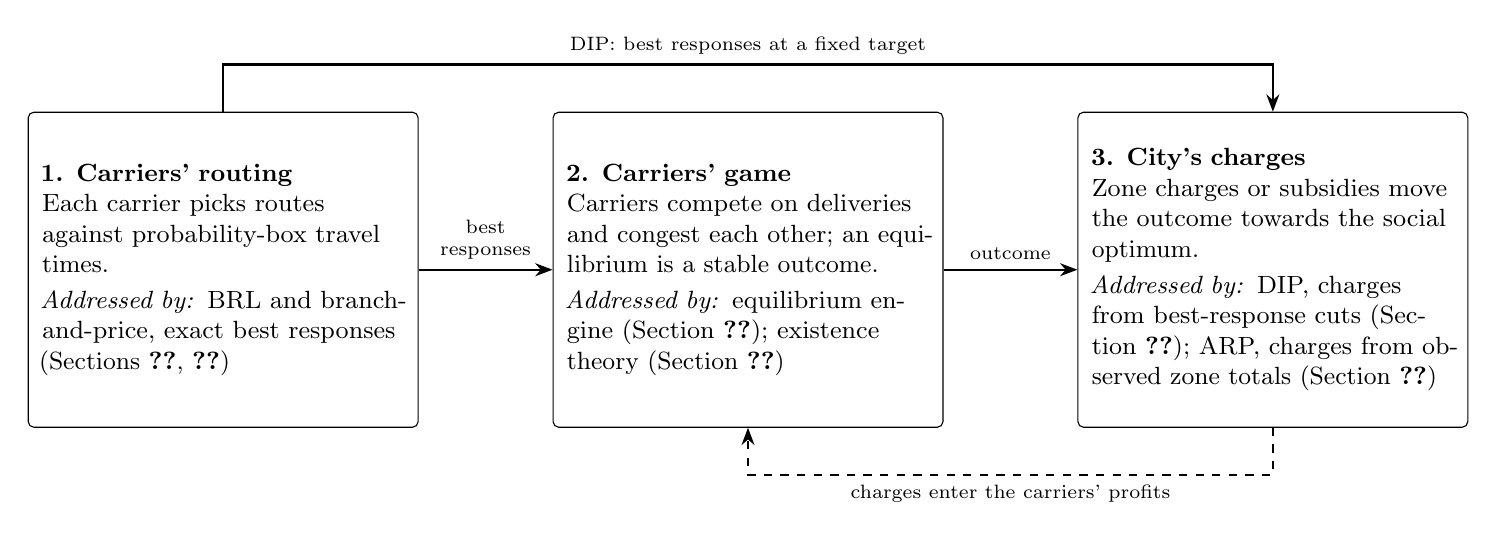
\begin{tikzpicture}[
  node distance=17mm,
  box/.style={draw, rounded corners=2pt, align=left, text width=4.6cm, minimum height=4.0cm, inner sep=5pt, font=\small},
  head/.style={font=\small\bfseries},
  arr/.style={-{Stealth[length=2.2mm]}, thick},
  lab/.style={font=\scriptsize, align=center}]
\node[box] (L1) at (0,0) {\textbf{1. Carriers' routing}\\ Each carrier picks routes against probability-box travel times.\\[2pt] \emph{Addressed by:} BRL and branch-and-price, exact best responses (Sections~\ref{sec:brl}, \ref{sec:bp})};
\node[box, right=of L1] (L2) {\textbf{2. Carriers' game}\\ Carriers compete on deliveries and congest each other; an equilibrium is a stable outcome.\\[2pt] \emph{Addressed by:} equilibrium engine (Section~\ref{sec:engine}); existence theory (Section~\ref{sec:theory})};
\node[box, right=of L2] (L3) {\textbf{3. City's charges}\\ Zone charges or subsidies move the outcome towards the social optimum.\\[2pt] \emph{Addressed by:} DIP, charges from best-response cuts (Section~\ref{sec:dip}); ARP, charges from observed zone totals (Section~\ref{sec:arp})};
\draw[arr] (L1.east) -- node[lab, above] {best\\responses} (L2.west);
\draw[arr] (L2.east) -- node[lab, above] {outcome} (L3.west);
\draw[arr] (L1.north) -- ++(0,6mm) -| node[lab, above, pos=0.25] {DIP: best responses at a fixed target} (L3.north);
\draw[arr, dashed] (L3.south) -- ++(0,-6mm) -| node[lab, below, pos=0.25] {charges enter the carriers' profits} (L2.south);
\end{tikzpicture}}
\caption{The three layers of the problem and the contribution that addresses each. Solid arrows show what is passed upward in the computation; the dashed arrow shows that the city's charges enter the carriers' profits.}\label{fig:layers}
\end{figure}

\paragraph{Contributions and their novelty level}
\begin{enumerate}[label=(\roman*),leftmargin=*,itemsep=0pt]
\item \emph{Model} (Section~\ref{sec:model}): a bilevel model with a public leader above carriers who choose routing plans, interact through zone aggregates of deliveries and vehicle-hours, and plan with probability-box travel times. The two congestion regimes, exposure and vehicle count, differ in their existence properties.
\item \emph{Budget-resource labelling (BRL)} (Section~\ref{sec:brl}): exact pricing of routes under probability boxes with unknown dependence. The comonotone worst case and the stop-loss decomposition \citep{Meilijson1979,Tchen1980} are known, and \citet{GhosalHoWiesemann2024} use the comonotone worst case for ambiguous demand in a capacity constraint. Here the per-arc budget of the decomposition becomes a decision resource of the pricing problem. Labels carry the route cost as a function of the budget and are pruned by a dominance rule restricted to a computable completion window, which we prove exact. With branch-and-price each carrier's integer plan is exact: all nine metropolitan instances are solved to proven optimality, with label sets \BrlLabNowinMetroMin--\BrlLabNowinMetroMax{} times smaller than without the window, with 22 customer zones in all nine cities and 30 to 40 customers in London and New York.
\item \emph{Leader pricing without equilibrium search} (Sections~\ref{sec:dip} and~\ref{sec:arp}). \emph{Dual implementation pricing (DIP)} computes a socially good target profile and then finds charges under which it is an equilibrium, by cutting planes whose separation step is one best response per carrier. \emph{Aggregate-response pricing (ARP)} lets the leader see only the zone aggregates of the market after each posted charge; in the convexified game its iteration contracts at a rate $\varrho=\max_z\kappa_z/(b_z+\kappa_z)$ that does not depend on the number of zones, carriers, lots, routing costs or probability boxes. The methods build on the Pigou--Cournot tax, toll polyhedra, inverse optimisation, trial-and-error tolls and marginal-contribution tariffs \citep{Buchanan1969,Bergendorff1997,Ahuja2001,Yang2004,Wolpert2001,Sandholm2002,Maheshwari2022}; the closest leader-side search, for nonatomic populations, is \citet{Masiha2026}. New here are the potential--welfare identity of the lumpy Cournot--congestion game with loss bounds, best responses of the carriers as the separation step, the instance-free rate, and the shift of the implementing charges under $\Gamma$-maximin beliefs.
\item \emph{Theory} (Section~\ref{sec:theory}): a credal absorption theorem. Above the explicit belief width $\sigma_{\max}\min\{N-1,\ d+1,\ 1+\sqrt{d\ln(2d)/2}\}$, a mixed equilibrium rounds to an exact pure imprecise equilibrium. The rounding step is the approximate-equilibrium result of \citet{Liu2023}; what is added is the explicit width and its reading under E-admissibility. Pure equilibria exist under exposure-based congestion, and deciding whether one exists is strongly NP-complete under vehicle-count congestion \citep{Apt2022,Gottlob2005}.
\item \emph{Evidence} (Sections~\ref{sec:data} and~\ref{sec:results}): nine metropolitan areas built from OpenStreetMap, gridded population and web-sourced operating parameters with quality grades; an exact integer oracle; ten random draws (seeds) of the city slice for New Delhi, Buenos Aires and London and nine for the other cities, with bootstrap confidence intervals; and the robustness of the game results to the carriers' criterion. The instance pipeline is released as a benchmark generator for multi-carrier routing games.
\end{enumerate}

\paragraph{Scope and organisation} The instances are stylised slices of nine cities with proxy demand, so the findings concern effects and orderings, not forecasts for a particular city. The levels of the price of anarchy, served share and leader gain describe carriers who plan against the guaranteed upper bound of the probability-box criterion; the orderings and policy directions carry over to carriers who plan with sample averages or Wasserstein balls, the levels do not (Section~\ref{sec:res-crit}). The leader's optimum is defined with optimistic equilibrium selection. Section~\ref{sec:related} places the work in the literature, Section~\ref{sec:model} defines the model, and Sections~\ref{sec:algo} and~\ref{sec:theory} give the algorithms and the equilibrium theory. Sections~\ref{sec:data} and~\ref{sec:results} describe the data and the computational study, and Sections~\ref{sec:discussion} and~\ref{sec:conclusion} discuss limits and conclude. Long proofs, extended data descriptions, the full per-city tables and further experiments are in a separate Supplementary Material, cited by section number (S1--S12) throughout. Each theorem is stated here with a proof sketch; the full statement and proof are in the Supplementary Material.

%======================================================================
\section{Related work}\label{sec:related}

\paragraph{Competing carriers and leaders above carriers} Carriers competing for requests have been studied by simulation \citep{Figliozzi2004}, with stylised games for shared collection points and lockers \citep{Li2024}, and in ride-hailing and crowdsourcing models with queues instead of routes \citep{Taylor2018,Benjaafar2022}. \citet{Cerulli2024} place a platform above carriers who solve profitable tour problems, but the carriers do not interact. Curb management supplies pricing leaders \citep{XuSun2024}, and collaborative routing \citep{GanstererHartl2018} gives savings that bound what cooperation could recover, not a price of anarchy. \citet{LiuMaMa2026} treat dynamic fleet routing with a non-cooperative game among agents with conflict penalties, solved by iterative best-response heuristics without a convergence guarantee; there is no pricing leader, no imprecise probabilities and no exact routing.

\paragraph{Routing under uncertainty} Robust and distributionally robust routing keeps the combinatorial structure when the ambiguity set is suitable \citep{Gounaris2013,GhosalWiesemann2020}. Closest to BRL, \citet{GhosalHoWiesemann2024} treat a capacitated routing problem with known travel times and ambiguous demand; the worst-case law is comonotone within each scenario, and the problem is solved by branch-and-cut, without pricing or labelling. Robust resource-constrained pricing by labelling is known for budgeted uncertainty sets \citep{Pessoa2015}. The comonotone worst case and the stop-loss decomposition are due to \citet{Meilijson1979} \citep[see also][]{Tchen1980}, and worst-case marginals of a probability box under monotone losses are standard \citep{Williamson1990}. None of these adds competition among carriers.

\paragraph{Games, aggregation and ambiguity} Potential and congestion games guarantee pure equilibria \citep{Rosenthal1973,Monderer1996}. A carrier chooses tours, so its strategy set is finite and nonconvex; \citet{Liu2023} prove, with a Shapley--Folkman argument \citep{Starr1969}, that nonconvex aggregative games have approximate pure equilibria whose error does not grow with the number of players. Equilibrium under ambiguous beliefs has been studied as equilibrium in beliefs \citep{Lo1996}, as robust-optimisation equilibrium \citep{Crespi2025} and with Wasserstein balls centred on the realised play \citep{Lanzetti2025,Feik2026}; \citet{Beauchene2016} treats ambiguous payoffs with accurate beliefs. For finite plan sets the worst-case criterion has no pure equilibrium in general, whereas an explicit belief width makes a rounded profile an exact equilibrium of the imprecise game. Deciding pure-equilibrium existence is NP-complete in polymatrix and integer programming games \citep{Apt2022,Carvalho2022} and hard for graphical games \citep{Gottlob2005}.

\paragraph{Tolls, implementation and adaptive pricing} Corrective taxes for market power and externalities go back to \citet{Buchanan1969} and \citet{Barnett1980}. Toll polyhedra that implement a target flow are classical for nonatomic routing \citep{Bergendorff1997}; the cutting-plane loop of DIP is an inverse-optimisation cutting plane \citep{Ahuja2001}, with best-response cuts as used for integer programming games \citep{Dragotto2023}. Marginal-contribution tariffs make welfare the potential of the game \citep{Wolpert2001,Marden2013}. Trial-and-error implementation of marginal-cost pricing from observed flows is due to \citet{Yang2004}, evolutionary implementation to \citet{Sandholm2002}, and adaptive incentive design with learning agents to \citet{Maheshwari2022,Maheshwari2026}. The closest leader-side method for combinatorial games \citep{Masiha2026} treats a nonatomic population and updates the leader's parameters by zeroth-order steps around a Wardrop solver; like a grid, it solves equilibria at every outer step, and it has no uncertainty and no atomic carriers. The novelty of each of our methods relative to these works is stated with the method, and the depth to which the neighbours were read is stated in Section~\ref{sec:discussion}.

%======================================================================
\section{Model}\label{sec:model}

Notation: $[n]=\{1,\dots,n\}$; $\ip{v}{w}$ is the inner product; $\|v\|_{w,\infty}=\max_k|v_k|/w_k$. Greek letters with related roles are kept apart: $\rho_j$ is an overtime rate, $\bar\rho$ a belief radius and $\varrho$ the contraction rate of ARP. The full model with all assumptions is in \SM{S1}.

\paragraph{Carriers, plans and congestion} The city is divided into zones $z\in[Z]$ and there are $N$ carriers. Carrier $i$ has a finite plan set $\cP_i$; a plan is a set of depot-to-depot routes over the carrier's customer zones. A plan $p$ determines deliveries $q_{iz}(p)$, vehicles $n_{iz}(p)$ and vehicle-hours $\tau_{iz}(p)$ in each zone, and a routing cost $C_i(p)$. Write $Q_z=\sum_iq_{iz}$ and $T_z=\sum_i\tau_{iz}$. Inverse demand in zone $z$ is $\alpha_z-b_zQ_z$ with $b_z>0$, and a vehicle-hour costs $\gamma(\xi_z+c_zX_z)$, where $\gamma>0$ is the hourly cost, $\xi_z$ the free-flow travel-time factor with mean $\mu_z$, $c_z>0$ the congestion slope and $X_z$ the congestion variable. The city charges $s_z$ per delivery and $t_z$ per unit of the congestion variable. Carrier $i$'s profit is
\begin{equation}\label{eq:profit}
u_i=\sum_z\big[q_{iz}(\alpha_z-b_zQ_z)-\gamma\tau_{iz}(\xi_z+c_zX_z)-s_zq_{iz}-t_zx_{iz}\big]-C_i(p).
\end{equation}
Two congestion regimes are distinguished: \textbf{D1 (exposure-based)}, $x_{iz}=\tau_{iz}$ and $X_z=\sum_i\tau_{iz}$, and \textbf{D2 (vehicle-count)}, $x_{iz}=n_{iz}$ and $X_z=\sum_in_{iz}$. Under D1 the carriers' interaction depends on the same quantity that determines the carrier's own congestion cost; under D2 the externality depends on counts rather than hours, which breaks the potential structure.

For the theory the interaction is written abstractly with $d=2Z$ coordinates $(z,Q)$ and $(z,X)$. Plan $p\in\cP_i$ has a contribution $a_i(p)\in\R^d_{\ge0}$ to the aggregate, an exposure $\varphi_i(p)\in\R^d_{\ge0}$ to the aggregate, a traffic exposure $t_i(p)\in\R^Z_{\ge0}$ and a private profit $\pi_i(p)$ (Assumption~A1 in \SM{S1}), and the coupling is affine: for a rival aggregate $m$ and traffic factor $\xi$, carrier $i$ obtains $u_i(p;m,\xi)=\pi_i(p)-\ip{\varphi_i(p)}{Mm}-\gamma\ip{t_i(p)}{\xi}$ with $M\ge0$ diagonal (Assumption~A2). Equation~\eqref{eq:profit} has this form. The game is \emph{of type D1} if $\varphi_i=a_i$ for all carriers and plans, and \emph{of type D2} otherwise. Social welfare, with charges treated as transfers, is
\begin{equation}\label{eq:welfare}
W(\sigma)=\sum_z\big[\alpha_zQ_z-\tfrac{b_z}{2}Q_z^2-\gamma\mu_zT_z-\gamma c_zT_zX_z\big]-\sum_iC_i(\sigma_i),
\end{equation}
and in the experiments the social cost is $\mathrm{SC}=-W$ with the traffic term part of the routing cost. The affine coupling excludes power-law congestion such as BPR curves, which we linearise (Section~\ref{sec:data}).

\paragraph{The routing layer}\label{sec:routing} For every arc $a$ the carrier knows a probability box: distribution functions $\Fl_a\le\Fu_a$ on a bounded support $[0,B_a]$, for example a Dvoretzky--Kiefer--Wolfowitz (DKW) band around the empirical distribution of $n$ observed days \citep{DKW1956}. The dependence between arcs is unknown, so the joint credal set is the Fr\'echet class $\cM$ of all laws whose $a$-th marginal lies between $\Fl_a$ and $\Fu_a$. A route of duration $T_r=\sum_{a\in r}X_a$ incurs a convex piecewise-linear loss
\begin{equation}\label{eq:loss}
\phi(T)=c_0+\gamma T+\textstyle\sum_{j=1}^{H}\rho_j\pos{T-\Theta_j},\qquad \gamma\ge0,\ \rho_j>0,\ 0\le\Theta_1<\dots<\Theta_H.
\end{equation}
In the experiments $H=1$: a fixed cost, an hourly cost and an overtime penalty after the shift length. The robust route cost is the upper prevision $\Eu[\phi(T_r)]=\sup_{P\in\cM}\E_P\phi(T_r)$, and $C_i(p)=\sum_{r\in p}\Eu[\phi(T_r)]$. A carrier's best response to prices on its deliveries and hours is a prize-collecting routing problem in which every route is priced by $\Eu[\phi]$. We call an exact solver of this problem the \emph{carrier oracle} (Assumption~A3 in \SM{S1}) and count \emph{oracle calls} as the cost unit of every method below.

\paragraph{The leader's problem} The city chooses charges $u$ from an admissible set $\mathcal U$. For a charge $u$ let $\mathrm{NE}(u)$ be the set of pure Nash equilibria of the carriers' game. With optimistic selection the leader's problem is
\begin{equation}\label{eq:bilevel}
\min_{u\in\mathcal U,\ \sigma}\ \mathrm{SC}(\sigma)\qquad\text{s.t.}\qquad\sigma\in\mathrm{NE}(u).
\end{equation}
The three leader methods compared in Section~\ref{sec:results} differ in what the leader may use: the \emph{grid} and DIP use the carriers' routing oracle, ARP uses only the zone aggregates the market produces after each posted charge.

%======================================================================
\section{Algorithms}\label{sec:algo}

The algorithms form a stack. BRL and branch-and-price implement the carrier oracle exactly. An equilibrium engine calls the oracle to compute a pure equilibrium for a given charge. DIP and ARP choose the charges; the grid baseline calls the engine once per grid point. Complete statements, Algorithms~1--3 and all proofs are in \SMs{S2 and S7--S10}.

\subsection{Budget-resource labelling (BRL)}\label{sec:brl}

\emph{In words.} A route is hard to price when the delays on its arcs could all be bad at the same time. Under unknown dependence the worst case is exactly that: every arc is equally unlucky at once. The route's cost then splits arc by arc once a time budget is allocated to each arc. BRL treats this budget as a resource in a shortest-path search. A partial route keeps its cost as a function of the budget, and it is dropped only if another partial route is at least as cheap for every budget that a completion can still use.

Let $\Qb_a(u)=\inf\{x:\Fl_a(x)\ge u\}$ be the upper quantile of arc $a$, $\xb_a=\int_0^1\Qb_a(u)\,du$ and $\Pib_a(d)=\int_0^1\pos{\Qb_a(u)-d}du$ the stop-loss transform of the lower distribution function.

\begin{theorem}[Upper prevision and budget decomposition]\label{thm:brl-main}
For every route $r$,
\[
\Eu[\phi(T_r)]=\int_0^1\phi\Big(\sum_{a\in r}\Qb_a(u)\Big)du
=c_0+\sum_{a\in r}\gamma\xb_a+\sum_{j=1}^{H}\rho_j\min\Big\{\sum_{a\in r}\Pib_a(d^j_a):\ \sum_{a\in r}d^j_a\le\Theta_j\Big\}.
\]
The supremum is attained by the comonotone coupling of the lower CDFs.
\end{theorem}
The first equality and the stop-loss identity are due to \citet{Meilijson1979}; we re-prove the statement (\SM{S8}) because the algorithm relies on the inequality-budget form and on integrality.

\begin{theorem}[Budget-resource reformulation]\label{thm:resource}
With dual prices $y$ and arc costs $c_a(d^1,\dots,d^H)=\gamma\xb_a+\sum_j\rho_j\Pib_a(d^j)$, the pricing problem $\min_{r}\{\Eu[\phi(T_r)]-\sum_{i\in r}y_i\}$ is an elementary shortest path problem in which every arc chooses a consumption $d^j_a$ of each of $H$ budget resources, paid through the separable convex cost $c_a$ and subject to $\sum_{a\in r}d^j_a\le\Theta_j$. The number of resources is $H$; it does not depend on the number of quantile levels $L$, the sample size or the number of arcs.
\end{theorem}

A scenario view of the same problem needs the $L$ level sums as resources and compares labels pointwise. BRL instead compares labels through their cost functions $f_p(D)$ of the budget $D$, but only where a completion can still reach. Let $C_{\min}(v)$ be a lower bound on the duration of any completion from the label's end node $v$ and define the completion window $\mathcal W(p)=[\Dl(p),\Dh(p)]$ with $\Dh(p)=\min\{S_{p,L},T_{\max}-C_{\min}(v)\}$ and $\Dl(p)=\min\{S_{p,1},\Dh(p)\}$, where $S_p$ is the level profile of the partial route and $T_{\max}$ the shift length.

\begin{definition}[Functional dominance]\label{def:fdom}
Label $p_1$ functionally dominates $p_2$, both ending at $v$, if $\mathcal V(p_1)\subseteq\mathcal V(p_2)$, $\ell(p_1)\le\ell(p_2)$ and $(f_{p_1}(D)-y(p_1))-(f_{p_2}(D)-y(p_2))\le0$ for all $D\in\mathcal W(p_2)$ ($\mathcal V$: visited set, $\ell$: load, $y$: collected duals).
\end{definition}

\begin{theorem}[Validity and exactness]\label{thm:fdom}
Functional dominance implies that every completion of $p_2$ is a completion of $p_1$ with no larger reduced cost. The labelling algorithm that discards dominated labels returns the minimum reduced cost exactly, with a route attaining it.
\end{theorem}

\emph{Sketch.} Concatenation of a label with a completion is an inf-convolution of their cost functions. The slope of $f_p$ lies in $[-\rho,0]$ and that of the completion's function in $[0,\rho]$, so an optimal split never lies above $\Dh(p)$, and below $S_{p,1}$ the difference of two label functions is nondecreasing; comparing on the window therefore loses no optimal completion (\SM{S8}). The test needs at most $2L+2$ evaluations. Quantile-vector and sector dominance are special cases of functional dominance, and neither converse holds. Under independent arc times concatenation is a convolution of laws rather than an inf-convolution and the method does not apply. Fixing a single risk level for all routes gives a lower bound but is not exact. Resource extension functions \citep{Irnich2008} are the general language for such pricing problems; BRL labels are functions of the budget joined by inf-convolution, and the window rests on the bounded slope of the loss, which that theory does not supply. Cost-function labels compared over a range of resource values are used for time-window problems with linear node costs \citep{Ioachim1998}, so we claim the window and its exactness proof for this loss, not the idea of comparing cost functions.

\subsection{Branch-and-price and the equilibrium engine}\label{sec:bp}\label{sec:engine}

Price-and-branch solves the integer problem only over the routes found at the root, so it can miss the integer optimum. We embed the BRL pricer in branch-and-price: set-partitioning (or prize-collecting set-packing) master with one column pool, column generation with the exact BRL pricer at every node, branching on the aggregated arc flow, a fleet-size row, ng-routes \citep{Baldacci2011} for the visited set (Theorem~\ref{thm:fdom} holds verbatim with the weaker relaxation), and a stop at relative gap $10^{-6}$. A zero gap proves optimality for the elementary problem. This is standard machinery; its purpose is to remove the inexact integer step (\SM{S2}).

For a given charge, the equilibrium engine starts from a zone-market-clearing (ZMC) guess and then lets the carriers best-respond one at a time, one oracle call each. Under D1 every improving move raises an exact potential, so the sequence ends at a pure equilibrium (Proposition~\ref{prop:D1}). ZMC has a clearing identity and a price-bracketing rate that does not depend on $d$, and on synthetic games it gave the smallest potential gap in \ZMCsynthWins{} of \ZMCsynthN{} instances; on the nine city games it did not beat plain best response (\SM{S11}). We use it as the starting phase of the engine and make no claim for it.

\subsection{Dual implementation pricing (DIP)}\label{sec:dip}

\emph{In words.} A city that could see everything would first pick the outcome it wants, the social optimum, and then look for charges under which the carriers choose it voluntarily. DIP does exactly this. It finds the charges by repeatedly asking each carrier what it would do instead (one best response) and adding a constraint that rules that deviation out. Because each question is one routing solve at a fixed target, no equilibrium has to be computed for any candidate charge.

\paragraph{Setting} We use the D1 instance in cost form. Carrier $i$ serves a subset of its customer zones with all-or-nothing lots $d_{iz}>0$, so $q_{iz}\in\{0,d_{iz}\}$; vehicle-hours are $\tau_{iz}=r\,q_{iz}$ for one ratio $r>0$; $R_i(p)\ge0$ is the robust routing cost of plan $p$; $g_z=\gamma c_z$. The city posts $s_z$ per delivery and $t_z$ per vehicle-hour. Write $\kappa_z=g_zr^2$, $m_z=b_z+\kappa_z$ and $\bar d_z$ for the mean lot in zone $z$. The social cost is $\mathrm{SC}(\sigma)=\sum_iR_i(\sigma_i)+\sum_z\big[-\alpha_zQ_z+\tfrac{b_z}{2}Q_z^2+g_zX_z^2\big]$. The game depends on the charges only through one number per zone, $u_z=s_z+rt_z$ (\SM{S2}, proposition ``One instrument per zone''), and every $u$ is realised by a uniform per-delivery charge plus non-negative zone congestion charges. The \emph{tangent charge} $u^{\tan}_z=\kappa_zQ^\circ_z-\tfrac{m_z}{2}\bar d_z$ at a target aggregate $Q^\circ$ is the classical corrective tax of a Cournot market with an externality, the marginal external damage at the target minus a market-power subsidy \citep{Buchanan1969,Barnett1980}. With all-or-nothing lots the subsidy is half a lot per delivery and includes the carriers' own congestion.

\begin{theorem}[Loss under asymmetric lots; exact implementation with symmetric lots]\label{thm:asym}\label{thm:convex}
In the convexified (mixed) game let $x^*$ minimise the convexified social cost $\overline{\mathrm{SC}}$, with aggregate $\bar Q^*$, and let $u=\kappa\odot\bar Q^*-\tfrac m2\odot\bar d$. Every convexified equilibrium $x^u$ satisfies $0\le\overline{\mathrm{SC}}(x^u)-\overline{\mathrm{SC}}(x^*)\le(1+\varrho)E$, where $\varrho=\max_z\kappa_z/m_z<1$ and $E=\sum_{i,z}\tfrac{m_z}{2}|d_{iz}-\bar d_z|\,d_{iz}$ measures how unequal the lots in a zone are. If all lots in a zone are equal, $E=0$: the tangent charge makes $x^*$ a convexified equilibrium and every convexified equilibrium under it has the optimal aggregate and social cost.
\end{theorem}
\emph{Sketch.} The potential of the game under charges $u$ equals the social cost up to a quadratic term in the aggregate, a term linear in the charge deviation $u-u^{\tan}$ and a lot-asymmetry term $L(\sigma)=\sum_{i,z}\tfrac{m_z}{2}(d_{iz}-\bar d_z)q_{iz}$ with $|L|\le E$ (the potential--welfare identity, \SM{S2}); comparing the identity at a potential minimiser with the expansion of $\overline{\mathrm{SC}}$ around $x^*$ bounds the deviation (\SM{S9}). A city cannot charge per carrier, which is why the loss of flat zone charges is measured. With carrier-specific charges every social optimum is an equilibrium; this is the classical marginal-contribution charge \citep{Wolpert2001,Marden2013}.

\paragraph{The pure game} For a pure target $\sigma^*$ and an admissible box $\mathcal U$ of charges, let $P(\sigma^*)=\{u\in\mathcal U:\ \ip{q_i(p)-q_i(\sigma^*_i)}{u}\ge J^0_i(\sigma^*_i;\sigma^*_{-i})-J^0_i(p;\sigma^*_{-i})\ \forall i,\forall p\in\mathcal P_i\}$, where $J^0_i$ is carrier $i$'s cost at zero charges. This is exactly the set of charges under which $\sigma^*$ is a pure Nash equilibrium: a polyhedron, possibly empty, of the kind that is classical for nonatomic routing \citep{Bergendorff1997,Ahuja2001}. Algorithm~\ref{alg:dip} searches it by cutting planes.

\begin{algorithm}[t]
\caption{DIP: dual implementation pricing}\label{alg:dip}
\begin{algorithmic}[1]
\State \textbf{Target.} Column generation on the convexified social cost, rounding and coordinate polish $\Rightarrow$ pure profile $\sigma^*$ with aggregate $Q^*$
\State \textbf{Reference.} $u^{\rm ref}\gets\kappa\odot Q^*-\tfrac m2\odot\bar d$; cuts $\mathcal C\gets\emptyset$; $u\gets u^{\rm ref}$
\Repeat
  \State for each $i$: $b_i\gets$ best response to $\sigma^*_{-i}$ under $u$ \Comment{$N$ routing calls, no equilibrium solve}
  \State for each $i$ with $J^u_i(b_i)<J^u_i(\sigma^*_i)$: add the violated constraint of $P(\sigma^*)$ for $(i,b_i)$ to $\mathcal C$
  \State \textbf{if} no cut was added: \Return $u$ \Comment{$\sigma^*$ is an exact pure equilibrium under $u$}
  \State $u\gets\arg\min\{\|u-u^{\rm ref}\|_1:u\in\mathcal U\text{ satisfies }\mathcal C\}$ (LP); \textbf{if} infeasible: \textbf{break}
\Until{}
\State \textbf{Fallback} (only if $P(\sigma^*)=\emptyset$): best-response dynamics from $\sigma^*$ under the least-violating charge and under $u^{\rm ref}$; keep the better equilibrium
\end{algorithmic}
\end{algorithm}

\begin{theorem}[Separation and finite termination]\label{thm:cut}
(a) $u\in P(\sigma^*)$ if and only if no carrier has a strictly improving best response to $\sigma^*_{-i}$ under $u$; an improving best response gives that carrier's most violated constraint. (b) With $\varepsilon=0$, Algorithm~\ref{alg:dip} stops after at most $1+\sum_i(|\mathcal P_i|-1)$ rounds, either with $u\in P(\sigma^*)$ or with an infeasible LP, which happens only if $P(\sigma^*)=\emptyset$. Each round costs $N$ oracle calls and no equilibrium solve.
\end{theorem}

\begin{proposition}[Single-level form]\label{prop:opt}
With optimistic selection the leader's value is $V^\star=\min\{\mathrm{SC}(\sigma):\sigma\text{ pure},\ P(\sigma)\ne\emptyset\}$. If Algorithm~\ref{alg:dip} ends in its main loop, the leader's loss is at most the suboptimality of the target, $\mathrm{SC}(\sigma^*)-\min_\sigma\mathrm{SC}(\sigma)$.
\end{proposition}

\begin{theorem}[Imprecision shifts the charge]\label{thm:credal}
Under $\Gamma$-maximin credal boxes of width $\delta$ (Lemma~\ref{lem:gamma}), the charges that implement $\sigma^*$ are $P(\sigma^*)-\hat s(\delta)$ with $\hat s_z(\delta)=\delta(b_zw_{(z,Q)}+r\,g_zw_{(z,X)})$. One run of DIP therefore gives $u(\delta)=u(0)-\hat s(\delta)$ for every width at no further oracle cost. For E-admissibility, maximality and interval dominance, $u(0)$ works at every width.
\end{theorem}

\begin{proposition}[When one instrument suffices]\label{prop:uniform}
A uniform per-delivery charge implements the convexified optimum under equal lots if the tangent charge is the same in every active zone. With the calibration of Section~\ref{sec:data} ($\alpha_z=1.5\,$fee, $b_z=\alpha_z/(2Q^{\rm full}_z)$) and $n_z$ carriers with equal lots in zone $z$, the congestion-free tangent charge is $u_z=-0.375\,\mathrm{fee}/n_z$: a subsidy of 37.5\% of the fee in single-carrier zones and 19\% in two-carrier zones.
\end{proposition}

\emph{Sketch of Theorem~\ref{thm:cut}.} Since $J^u_i=J^0_i+\ip{u}{q_i}$, membership in $P(\sigma^*)$ is exactly the absence of a profitable unilateral deviation, so the separation oracle is a best response at the fixed target, not an equilibrium solve. The LP over the cuts has no repeated cut, which bounds the number of rounds by the number of plans (\SM{S9}). Selection remains optimistic: the target is an exact equilibrium under the returned charges, but other equilibria may coexist. DIP combines the Pigou--Cournot tax, marginal-contribution utilities, toll polyhedra and best-response cuts cited above; new are the exact potential--welfare identity of the lumpy Cournot--congestion game with loss bounds in $E$, the translation of the implementing charges by the $\Gamma$-maximin surcharge, and the competitor-count rule of Proposition~\ref{prop:uniform}. The bound on the loss of the fallback, the oracle-call count and the proofs are in \SMs{S2 and S9}.

\subsection{Aggregate-response pricing (ARP)}\label{sec:arp}

\emph{In words.} ARP asks what a city can do without the carriers' routing models. It posts a charge, watches the zone totals that the carriers then deliver, and moves each zone's charge towards the corrective tax that those totals imply. In the convexified game this update is a contraction, so the iteration settles at a rate that depends only on the demand and congestion slopes, not on the number of carriers or on how hard their routing problems are.

The city knows its own demand and congestion slopes $(b,g,r)$ and hence $\kappa_z$ and $m_z$. It posts a per-delivery-equivalent charge $u\in\R^Z$, the carriers settle in a pure equilibrium by their own best responses, and the city observes the deliveries $Q_z$ and the number $n_z$ of active carriers in each zone, nothing else. With an estimate $\bar d_z$ of the mean lot (from $Q_z/n_z$; a jump of $Q_z$ when $n_z$ changes by one is the lot of the carrier that entered or left) the \emph{flat rule} updates
\begin{equation}\label{eq:rule}
u^{t+1}_z=(1-\theta_z)u^t_z+\theta_z\big[\kappa_zQ^t_z-\tfrac{m_z}{2}\bar d_z\big],\qquad\theta_z\in(0,1].
\end{equation}
With $\theta=1$ this is DIP's tangent charge evaluated at the observed aggregate instead of a computed target. The iteration stops at a fixed point or when the posted charge and market state repeat (a cycle). A \emph{marginal tariff} (ARP-M) bills each carrier the exact externality of its lot on the others and its market-power wedge, $T_z(q_{iz},Q_z)=\kappa_zq_{iz}(Q_z-q_{iz})-\tfrac{b_z}{2}q_{iz}^2$, a function of the carrier's own deliveries and the zone total only.

\begin{theorem}[Marginal tariff; the mechanism is classical]\label{thm:mct}
Under the tariff $T_z$ in every zone, (a) $J^T_i(p;\sigma_{-i})=\mathrm{SC}(p,\sigma_{-i})-\mathrm{SC}(\emptyset_i,\sigma_{-i})$, so $\mathrm{SC}$ is an exact potential of the tariff game; (b) the pure equilibria are exactly the profiles that no single carrier can improve socially, every social optimum is a pure equilibrium, and best-response dynamics from any profile never increase $\mathrm{SC}$; (c) a best response is one oracle call with the zone prices shifted by $\kappa_zQ_{-i,z}-\tfrac{b_z}{2}d_{iz}$.
\end{theorem}
The mechanism is the marginal-contribution tariff of \citet{Wolpert2001}, \citet{Sandholm2002} and \citet{Marden2013}; what is stated here is its lumpy form in the city game. It leaves equilibrium selection open: the dynamics stop at a unilateral social optimum, which may be a local optimum of $\mathrm{SC}$.

\paragraph{Theory of the flat rule} Convexify the plan sets and let $\bar Q(x)$ be the aggregate of a mixed profile. Let $F$ be the carriers' aggregate value function plus the social-cost terms in $Q$, defined in \SM{S2}.

\begin{theorem}[The response is a proximal map; instance-free contraction]\label{thm:resolvent}\label{thm:rate}
$F$ is $1$-strongly convex in $\|\cdot\|_m$. For every charge $u$ all convexified equilibria share one aggregate $Q(u)=\arg\min_Q\{F(Q)+\ip uQ\}$, and $\|Q(u_1)-Q(u_2)\|_m\le\|u_1-u_2\|_{m^{-1}}$. The leader's problem is the Fenchel dual $\min_uD(u)$, whose gradient is observable from the aggregate alone; its unique minimiser $u^*$ is the unique fixed point of $u\mapsto\kappa\odot Q(u)-\tfrac m2\odot\bar d$, and with symmetric lots it implements a convexified social optimum (in general within $E_{\bar d}$ of one). Let $\varrho=\max_z\kappa_z/m_z<1$. (a) The plain rule ($\theta=1$) satisfies $\|u^{t+1}-u^*\|_{\kappa^{-1}}\le\varrho\|u^t-u^*\|_{\kappa^{-1}}$; (b) the damped rule with $\theta=2/(2+\varrho)$ contracts at ratio $\varrho/(2+\varrho)<1/3$. The ratios depend on the instance only through $\varrho$, not on $Z$, $N$, the number of customers, the lots, the routing costs or the probability boxes.
\end{theorem}
\emph{Sketch.} Strong convexity of $F$ makes the carriers' aggregate response the proximal (resolvent) map of $F$, which is non-expansive in the dual norm; the flat rule is gradient descent on $D$ in the $\kappa^{-1}$ geometry, and the Cournot slope $b_z$ makes the step a contraction with constant $\varrho$ (\SM{S10}). Without the demand side ($b=0$), $\varrho=1$ and there is no contraction, which is why the nonatomic literature uses averaging \citep{Yang2004}. The identification of the response as a proximal map with instance-free rates in a lumpy NP-hard routing game is the new part.

\begin{proposition}[Pure game and imprecise carriers]\label{thm:pure}\label{prop:arpcredal}
(a) At a pure equilibrium under the fixed-point charge with symmetric lots, no carrier can lower the social cost unilaterally. (b) If the observed aggregate differs from the convexified response by $e^t$, then $\|u^{t+1}-u^*\|_{\kappa^{-1}}\le\varrho\|u^t-u^*\|_{\kappa^{-1}}+\|e^t\|_\kappa$; this bound is conditional on the carriers settling at potential minimisers. (c) The convexified response determines $F$ up to a constant, so the convexified optimum is all that an observation-only scheme can target; the pure social optimum is not identified. (d) Under $\Gamma$-maximin beliefs of width $\delta$ the response to $u$ is the precise response to $u+\hat s(\delta)$, so the flat rule needs no knowledge of $\delta$, contracts at the same rates and only moves its fixed point.
\end{proposition}
ARP follows trial-and-error marginal-cost pricing \citep{Yang2004,HanYang2009,YeYangTan2015}, evolutionary implementation of pricing \citep{Sandholm2002} and adaptive incentive design \citep{Maheshwari2022,Maheshwari2026}, whose fixed points are socially optimal; \citet{Masiha2026} give a model-free zeroth-order loop with stationarity rather than a rate. Proofs and the full statements are in \SM{S10}.

%======================================================================
\section{Equilibrium theory}\label{sec:theory}

This section states the results on pure and imprecise equilibria; full statements are in \SM{S3} and proofs in \SM{S7}. Results labelled \emph{classical} are known and cited.

\emph{In words.} When carriers choose among a few discrete plans, an equilibrium in pure plans, the kind a city can observe, need not exist. We show when it does (exposure-based congestion) and when deciding existence is hard (vehicle-count congestion). We also show that a carrier who is unsure about its rivals' activity by an explicit margin accepts a rounded version of a mixed equilibrium as an exact equilibrium of its imprecise game.

\paragraph{Imprecise beliefs} Fix weights $w\in\R^d_{>0}$ and a width $\delta\ge0$. At a pure profile $\sigma$, carrier $i$'s credal set $\cM_i^\delta(\sigma)$ is the set of Borel laws on the rival aggregate $m\in\R^d_{\ge0}$ and traffic factor $\xi$ with finite first moments such that $\E[m]$ lies in the box $K^\delta(A_{-i}(\sigma))=\{m\ge0:|m_k-A_{-i,k}|\le\delta w_k\}$ centred at the realised rival aggregate $A_{-i}(\sigma)$ (the consistency requirement of equilibrium in beliefs, \citealp{Lo1996}) and $\E[\xi]$ lies in a traffic box $\Xi$. A plan is \emph{E-admissible} if it maximises expected payoff for some law in the credal set, \emph{maximal} if no other plan has a strictly positive lower expected advantage, \emph{interval-undominated} (ID) if its upper expectation is at least the best lower expectation, and \emph{$\Gamma$-maximin} if it maximises the lower expectation \citep{Troffaes2007}. $\ICNE_C(\delta)$, for $C\in\{E,M,ID,\Gamma\}$, is the set of pure profiles in which every carrier's plan is $C$-admissible; $\delta_0^C$ is the smallest width with $\ICNE_C(\delta)\neq\emptyset$. Under the affine coupling every criterion depends on the credal set only through its mean box, and $\ICNE_E(\delta)\subseteq\ICNE_M(\delta)\subseteq\ICNE_{ID}(\delta)$ with monotonicity in $\delta$ (\SM{S3}).

\begin{lemma}[$\Gamma$-maximin surcharge]\label{lem:gamma}
If $\varphi_i(p),t_i(p)\ge0$, the lower expectation over the credal box is attained, for every plan simultaneously, at the upper corner (rival aggregate $A_{-i}+\delta w$, traffic $\overline\mu$). Consequently $\ICNE_\Gamma(\delta)$ is the set of pure Nash equilibria of a precise game with private profits $\pi_i^\Gamma(p)=\pi_i(p)-\delta\ip{\varphi_i(p)}{Mw}-\gamma\ip{t_i(p)}{\overline\mu}$.
\end{lemma}
The surcharge is what a cautious carrier adds to the cost of activity in zone $k$ because it fears up to $\delta w_k$ more rival activity than it observes.

\begin{proposition}[Existence under D1 at every width]\label{prop:D1}
Under D1, for every traffic $\hat\xi\in\Xi$, $\Psi_{\hat\xi}(\sigma)=\sum_i\big[\pi_i(\sigma_i)+\tfrac12\|a_i(\sigma_i)\|_M^2-\gamma\ip{t_i(\sigma_i)}{\hat\xi}\big]-\tfrac12\|A(\sigma)\|_M^2$ is an exact potential of the precise game. Every maximiser lies in $\ICNE_E(\delta)$ for all $\delta\ge0$, so $\delta_0^E=\delta_0^M=\delta_0^{ID}=0$, and $\ICNE_\Gamma(\delta)\neq\emptyset$ for all $\delta\ge0$.
\end{proposition}
\emph{Sketch.} For a unilateral change of carrier $i$ from contribution $a$ to $a'$ against rival aggregate $R$, the quadratic terms give $-\ip{a'-a}{MR}$, which equals the change of the coupling term when $\varphi_i=a_i$. A maximiser of an exact potential is a pure equilibrium \citep{Monderer1996}, and the centre of every credal box is the realised aggregate. For $\Gamma$, the surcharge game is again of type D1.

\paragraph{Credal absorption} Let $x^*$ be a mixed equilibrium of the precise game (it exists by Nash's theorem; under affine coupling, mixed equilibria are exactly the profiles in which every plan in the support is a best response to the mean rival aggregate). Write $B_j$ for carrier $j$'s best-response set at $x^*$, $\bar a_j$ for its mean contribution, $\bar\sigma=\max_{j,k}\max_{p,p'\in B_j}|a_{jk}(p)-a_{jk}(p')|/w_k$ for the largest spread, $\bar\rho$ for the largest deviation of a best-response contribution from its mean (in units $w_k$), $d_L$ for the dimension spanned by the contribution differences and $k^\sharp=\min\{N,d_L\}$, and $\sigma_{\max}=\max_{i,k}\operatorname{range}_{p\in\cP_i}a_{ik}(p)/w_k$, so $\bar\rho\le\bar\sigma\le\sigma_{\max}$. The \emph{anchored radius} of a pure profile $p\in\prod_jB_j$ is $\hat\delta(p)=\max_i\|A_{-i}(p)-\sum_{j\ne i}\bar a_j\|_{w,\infty}$.

\begin{theorem}[Credal absorption]\label{thm:main}
Under the affine coupling and with $x^*$ as above:
(a) \emph{Absorption.} For every $p\in\prod_jB_j$ and every $\delta\ge\hat\delta(p)$, $p\in\ICNE_E(\delta)\subseteq\ICNE_M(\delta)\subseteq\ICNE_{ID}(\delta)$.
(b) \emph{Radius.} $\min_{p\in\prod_jB_j}\hat\delta(p)\le\min\big\{(N-1)\bar\rho,\ k^\sharp\bar\sigma+\bar\rho,\ \bar\sigma\sqrt{k^\sharp\ln(2d)/2}+\bar\rho\big\}$, where the first term can be sharpened to $\max_{i,k}\sum_{j\ne i}r_{jk}/w_k$.
(c) \emph{Uniform existence.} $\delta_0^{ID}\le\delta_0^M\le\delta_0^E\le\sigma_{\max}\min\{N-1,\ d+1,\ 1+\sqrt{d\ln(2d)/2}\}$.
(d) \emph{Construction.} A profile achieving the second bound is obtained from $x^*$ by one linear program (a vertex of the polytope of Shapley--Folkman decompositions) followed by an arbitrary choice for at most $k^\sharp$ carriers; the third by independent sampling of these carriers.
\end{theorem}
\emph{Sketch.} Every carrier in $p\in\prod_jB_j$ plays a best response to the \emph{anchor} $\sum_{j\ne i}\bar a_j$. If $\delta\ge\hat\delta(p)$, the anchor lies in the clipped box around the realised aggregate, so the Dirac law at the anchor belongs to the credal set and witnesses E-admissibility. The radius bounds follow from a Shapley--Folkman decomposition in which at most $k^\sharp$ carriers remain mixed; the remaining sum is bounded deterministically or, after independent sampling, by Hoeffding's inequality and a union bound. The own term $a_i(p_i)-\bar a_i$ cannot be removed (the ``$+1$'' in the bound of \citealp{Liu2023}). A corollary shows that such a profile is an $\varepsilon$-Nash equilibrium of the precise game.

\emph{Regime and relation to prior work.} On the city instances $N\le6$ and $d=2Z\ge84$, so the Shapley--Folkman step selects nothing and the applicable term is the support-selection bound $(N-1)\bar\rho$, which grows with $N$; its $N-1$ factor is attained at $N=2$ and a dependence on the number of zones is necessary (\SM{S3}). The terms $d+1$ and $1+\sqrt{d\ln(2d)/2}$ are smaller than $N-1$ only when $N>d$, for example with per-vehicle or crowdsourced players; the $N$-uniform bound is not shown to be attained. The approximate equilibrium and part (a) are in \citet{Liu2023}, and we claim no novelty for either; the addition is the explicit belief box and the reading that, under E-admissibility, the belief width absorbs the rounding error. $\Gamma$-maximin beliefs reduce to a precise surcharge game (Lemma~\ref{lem:gamma}), so absorption does not apply to them and under D2 that set can be empty. Further results in \SM{S3} show that imprecise equilibria are approximate equilibria of the precise game, that price-of-anarchy and stability curves are monotone in the belief width, and that a smoothness bound transfers conditionally; the price-of-anarchy values in Section~\ref{sec:results} are empirical.

\begin{theorem}[NP-completeness under D2]\label{thm:np}
Deciding $\ICNE_C(\delta)\neq\emptyset$ for a game given by explicit plan lists with rational data is in NP for each $C\in\{E,M,ID,\Gamma\}$. For every digraph $D$ with maximum out-degree $\Delta^+\ge1$ one constructs in polynomial time a D2 instance with two plans per carrier and one zone per arc such that, for all $\delta\in[0,1/(2\Delta^++1))$, $\ICNE_E(\delta)=\ICNE_M(\delta)=\ICNE_{ID}(\delta)=\ICNE_\Gamma(\delta)$ is the set of profiles that play ``in'' exactly on a kernel of $D$. Hence the problem is strongly NP-complete for each criterion, already at $\delta=0$, and for every fixed $\delta\in[0,1/5)$; unless $\mathrm P=\mathrm{NP}$, no polynomial algorithm approximates $\delta_0^E$ of a D2 instance within any fixed factor.
\end{theorem}
\emph{Sketch.} Deciding whether a digraph has a kernel is NP-complete \citep{Chvatal1973,Fraenkel1981}. Each vertex becomes a carrier with an ``out'' plan of zero data and an ``in'' plan that puts one vehicle on each out-arc zone and two on each in-arc zone. The gain of ``in'' is positive if no out-neighbour plays ``in'' and at most $-1$ otherwise, and the sign is constant on every credal box of width below $1/(2\Delta^++1)$, so all four criteria select the realised strict best response. Pure-equilibrium existence is known to be NP-complete in polymatrix and integer programming games \citep{Apt2022,Carvalho2022}; this is a kernel reduction specialised to the rank-one D2 structure and extended to four credal criteria. Together with Proposition~\ref{prop:D1} it gives a complexity split between the two congestion regimes: exposure-based congestion yields a potential game with guaranteed pure imprecise equilibria, vehicle counting does not. Under D2 the mixed equilibrium that Theorem~\ref{thm:main} rounds is itself PPAD-hard to compute \citep{Chen2009,Daskalakis2009}.

\paragraph{Thresholds, rounding and machine-checked statements} For any pure profile the exact E-threshold is the value of a linear program over the box, and Theorem~\ref{thm:main} together with this computation defines a four-phase rounding algorithm (relax, sparsify, round, compute the exact width; \SM{S3}). It was not run on the city games, which use the D1 engine; the exact thresholds were used in the tests of Section~\ref{sec:res-theory}. With power-law congestion the credal statements fail; we do not treat that case. The repository contains a Lean~4 development that checks the finite or algebraic cores of several results (credal results, the D1 potential identity, parts of DIP, the marginal tariff, ARP and BRL); it does not formalise probability boxes, convex conjugates, the Hoeffding term, NP-completeness or any computation (\SM{S12}).

%======================================================================
\section{Data and calibration}\label{sec:data}

\paragraph{Road networks and zones} For each of nine cities (New Delhi, Cairo, Moscow, Buenos Aires, New York, Mumbai, London, Paris, Berlin) we use an OpenStreetMap extract \citep{Haklay2008} distributed by BBBike (replication timestamp 16 October 2026). The drivable major-road network is kept as an undirected graph with class-based free-flow speeds and lane counts. Population comes from the GHS-POP R2023A grid, epoch 2025, at 30 arc-seconds \citep{GHSPOP2023}. Zones are blocks of $4\times4$ raster cells (about 3.7\,km) with at least one inhabitant; zone-to-zone free-flow times are shortest paths between population-weighted centroids plus a fixed access time. Points of interest give a depot score per zone used to place carrier depots. Table~\ref{tab:cities} summarises the instances; $Z$ ranges from \Zmin{} to \Zmax. Details are in \SM{S4}.

\begin{table}[tbp]\centering\small
\caption{City instances. $Z$: zones; population from GHS-POP inside the zones; major road and lane kilometres inside the zones; nodes of the major-road graph; $N$: number of carriers.}\label{tab:cities}
\adjustbox{max width=\linewidth}{\begin{tabular}{lrrrrrr}
\toprule
City & $Z$ & pop.\ (M) & major road km & lane-km & graph nodes & $N$ \\
\midrule
New Delhi & 120 & 25.0 & 5\,556 & 8\,590 & 138\,542 & 5 \\
Cairo & 42 & 14.9 & 2\,649 & 4\,498 & 119\,027 & 4 \\
Moscow & 160 & 12.6 & 4\,475 & 12\,325 & 146\,234 & 5 \\
Buenos Aires & 208 & 13.3 & 5\,764 & 12\,032 & 130\,526 & 4 \\
New York & 234 & 12.1 & 8\,798 & 17\,770 & 382\,014 & 4 \\
Mumbai & 143 & 22.0 & 4\,259 & 7\,092 & 109\,804 & 5 \\
London & 348 & 11.3 & 7\,110 & 13\,628 & 350\,931 & 5 \\
Paris & 198 & 9.02 & 5\,990 & 10\,854 & 309\,175 & 5 \\
Berlin & 593 & 4.65 & 5\,490 & 11\,147 & 192\,577 & 6 \\
\bottomrule
\end{tabular}
}
\end{table}

\paragraph{Operating parameters and grades} Per-city parameters were collected from public web sources on 23 October 2026 and graded A (official or primary statistic), B (industry report or country-level proxy) or C (rough estimate or proxy from elsewhere). The values used and the grade of each are in \SM{S4} (Table~S-params), and the repository file \texttt{data/parameters/SOURCES.md} gives source, URL, grade and note for each number. Congestion levels are those of the TomTom Traffic Index 2025 \citep{TomTom2025}; volume-delay curves use the BPR form with $\alpha=0.15$, $\beta=4$ \citep{BPR1964}, linearised at the observed congestion level. The weak numbers are: parcels per capita (country-level), driver wages (minimum-wage floors or job-site averages), drops per vehicle and van capacities outside the United States (proxies), delivery fees in Cairo, Moscow and Buenos Aires (consumer or reference rates), market shares (available only for Paris and Berlin; elsewhere equal shares) and Moscow's congestion level (2020). The sensitivity of the equilibria to the five weakest parameters is in \SM{S4}.

\paragraph{Calibration rules and simplifications} Each carrier serves 22 customer zones sampled around its depot with weight proportional to population times a gravity decay in travel time, so carriers overlap in some zones. A lot is 10--50\% of a vehicle's daily drops, proportional to the zone's parcel demand. Inverse demand has intercept $\alpha_z=1.5\times$ fee and slope $b_z=\alpha_z/(2Q_z^{\rm full})$. The congestion slope $c_z$ is the derivative of the BPR curve at the TomTom level, scaled by a slice multiplicity $\varsigma_z$ so that the slice faces the congestion of the whole city. Travel-time multipliers of nine sectors follow a lognormal law matching the TomTom congestion; each carrier observes 30 days, from which DKW boxes at confidence $1-\alpha$ are built. The route loss \eqref{eq:loss} uses the vehicle-hour cost per hour, twice that as fixed cost, three times that per overtime hour, and the shift length as deadline. The simplifications are:
(S1) all-or-nothing lots, which make the Cournot game lumpy; (S2) the integer routing step: the main game experiments use branch-and-price with a time limit per call, while the engine comparison and some checks use price-and-branch; (S3) vehicle-hours proportional to the lot, so within a zone a congestion charge on hours and a delivery charge are collinear; (S4) linear congestion (D1); (S5) oracle exactness at city scale is checked against an independent oracle, not proved. A \emph{broad} social cost that adds the delay imposed on background traffic is reported in \SM{S5} but not used for conclusions. The instance pipeline is released and regenerates all instances from the raw extracts; the instances are small (22 customer zones per carrier, four to six carriers) so that exact oracles are possible, and are intended as a test bed for algorithms on multi-carrier routing games, not as validated city models.

%======================================================================
\section{Computational study}\label{sec:results}

The study addresses seven questions: is BRL pricing exact and how far does branch-and-price scale (Section~\ref{sec:res-brl}); why probability boxes (Section~\ref{sec:res-pbox}); how the equilibria, price of anarchy and imprecision look on the nine cities (Section~\ref{sec:res-eq}); how DIP and ARP compare with the grid and with the social optimum in calls and gain (Section~\ref{sec:res-leader}); whether the findings are robust to the carriers' criterion (Section~\ref{sec:res-crit}); whether the theory holds on the city equilibria (Section~\ref{sec:res-theory}); and how the equilibria were verified (Section~\ref{sec:res-verif}). Details, per-city tables and further experiments are in \SM{S5} and \SM{S6}.

\paragraph{Protocol and seeds} All numbers are generated from the result files of the repository by \texttt{make\_tables.py}. A seed redraws the depots, the customer zones of each carrier, the travel-time sectors and the 30 observed days, hence the probability boxes; calibration inputs are the same in every seed. Seeds 0--2 were run for all nine cities and the exact-oracle study was extended to seeds 3--9, which used \TenOracleCalls{} oracle calls, of which \TenUnprovenPct\% were not proven optimal. Coverage: \TenFullCities{} have ten seeds for everything, including the full 63-point exact grid and ARP; \TenRedCities{} have \TenRedSeedsMax{} seeds (0--8) for the unpriced equilibrium, the social optimum, the price of anarchy and DIP, while grid-derived quantities still have three seeds and a reduced exact grid (\ExEtwoRedMin--\ExEtwoRedMax{} screened points per seed), so they are lower bounds (marked $^*$); imprecision sweeps and the criterion study use three seeds. Means over seeds are given with percentile bootstrap 95\% confidence intervals (10{,}000 resamples of the seeds). They describe the spread over sampled slices of a city, not the uncertainty in the calibration inputs. Of the \ExCalls{} oracle calls of the seeds 0--2 study, \ExProvenPct\% were proven optimal, and the remaining gap of an unproven call was at most \ExMaxGap{} USD.

%----------------------------------------------------------------------
\subsection{BRL and branch-and-price}\label{sec:res-brl}

\paragraph{Exactness} The upper-prevision formula agrees with a linear program over all joint laws on \BRLtestAn{} random instances to a relative error of \BRLtestAerr; the comonotone worst case exceeds the value under independent worst marginals by \BRLindepMean\% on average and up to \BRLindepMax\%. BRL pricing equals complete enumeration on every test instance, including \BRLrealCmatch{} of \BRLrealCn{} sub-instances built from the nine cities. Fixing one risk level for all routes is suboptimal in \BRLfixeduSub{} of \BRLfixeduN{} small exact comparisons, by up to \BRLfixeduMax\%.

\paragraph{What BRL does well} With the duals of the root column generation, the window rule keeps \BrlLabNowinMetroMin--\BrlLabNowinMetroMax{} times fewer labels than the same stop-loss comparison without the window, and \BrlLabQvMetroMin--\BrlLabQvMetroMax{} times fewer than quantile-vector dominance on the metro instances (22--80 customer zones); on public benchmark instances (Solomon and Augerat, treated as capacitated routing with a soft duration limit and four sectors, an emulation and not a reproduction of published branch-and-cut results) the factors are \BrlLabNowinPubMin--\BrlLabNowinPubMax{} and \BrlLabQvPubMin--\BrlLabQvPubMax. The ratios shrink as $n$ grows, and the reductions on real data are smaller than on random instances. On the nine metro instances with 22 customer zones, branch-and-price proved optimality in \BPoptimalN{} of nine cities, in at most \BPtimeMaxMin{} minutes on one core (\BPtimeMaxCity, \BPnodesMax{} nodes). Against complete enumeration on \BPverN{} random formulations, branch-and-price returned the optimum in \BPverExact{} of \BPverN, whereas price-and-branch was strictly suboptimal in \BPverPBsub{} of them, by up to \BPverPBmax\%. The scale study gives proofs for Cairo, London and New York at 30 zones, and for London at 40 zones (and for New York at 40 zones with the device configuration). We have not run a general resource-extension-function or function-label labelling code \citep{Dabia2013} against the completion window.

\paragraph{What BRL does not do} On held-out days from the same law, BRL does not beat the sample-average plan: its plans cost \BrlOosMeanMin--\BrlOosMeanMax\% more on the mean and \BrlOosPNineFiveMin--\BrlOosPNineFiveMax\% more at the 95th percentile after polishing. Only in a stress test, with a law shifted away from the training days and ten training days, is BRL's 95th percentile \BrlShiftTenPNineFive\% lower and its CVaR$_{0.9}$ \BrlShiftTenCvar\% lower, at \BrlShiftTenMean\% more on the mean; the advantage vanishes at 30 or more days. BRL's advantage is thus proof speed and label counts against scenario and quantile labelling, not out-of-sample cost. BRL was proven in only \BrlAugeratProvenN{} of \BrlAugeratCells{} Augerat cells, and optimality was not proven at London with 60 or 80 zones or New Delhi with 60. The method should therefore be read as exact where proven (22 customer zones in all nine cities, 30 to 40 customers in London and New York) and not beyond about 40 customers. On the metro instances the robust optimum is not the best plan under the calibrated law: the branch-and-price plan is worse than the sample-average plan in \BPtrueWorse, and its worst-case cost lies between \BPconsMin\% and \BPconsMax\% above its expected cost under the law.

%----------------------------------------------------------------------
\subsection{Why probability boxes}\label{sec:res-pbox}

We compared the criteria out of sample on the nine metro instances (seed 0, 22 customer zones) against sample-average approximation (SAA), a type-1 Wasserstein ball and CVaR, with $n=10,20,30,60$ training days, \AmbDraws{} independent draws, and a held-out set of 20{,}000 days. The planner is a heuristic validated against branch-and-price: optimal in \AmbValOptN{} of \AmbValRows{} instances, at most \AmbValMaxGap\% above in the others. \emph{The p-box loses in expected cost.} At every $n\le60$ its regret is \AmbRegMin--\AmbRegMax\%, against \AmbSaaRegTwoZero\% for SAA at $n=20$ and \AmbSaaRegSixZero\% at $n=60$; Wasserstein with a cross-validated radius reproduces SAA, and CVaR$_{0.9}$ costs \AmbCvarRegTwoZero\% and \AmbCvarRegSixZero\%. The cost comes from the DKW band, not from the unknown-dependence worst case. \emph{It buys tail protection and a bound.} At $n=20$ the probability of an overtime day is \AmbOtSaaTwoZero{} for SAA and \AmbOtPbTwoZero{} for the p-box with confidence 0.80, and the CVaR$_{0.95}$ of the daily cost is \AmbCvarGainLo--\AmbCvarGainHi{} percentage points lower than under SAA at every $n$. The criterion value is an upper bound on the true expected cost whenever the DKW band holds: it exceeds the realised cost by \AmbDisPbMin--\AmbDisPbMax\% for the p-box, by \AmbDisWcvTwoZero\% for the cross-validated Wasserstein criterion and by \AmbDisSaaTwoZero\% for SAA at $n=20$. P-boxes thus do not minimise expected cost; they provide a guaranteed upper bound that shrinks with the sample size, and tail protection, at an expected-cost price of \AmbRegMin--\AmbRegMax\% for $n\le60$ (\SM{S5}, Table~S-ambig).

%----------------------------------------------------------------------
\subsection{Unpriced equilibria, price of anarchy and imprecision}\label{sec:res-eq}\label{sec:res-poa}\label{sec:res-engine}

The cities fall into two groups (\SM{S5}, seeds 0--2, exact oracle). In \EoneHighCities{} the carriers serve at least \EoneServedHighMin\% of customer demand; in \EoneLowCities{} they serve \EoneServedLowMin--\EoneServedLowMax\%, because the delivery fee is low relative to the vehicle-hour cost or the shift is short. The added slowdown caused by delivery vehicles is \EoneSlowMin--\EoneSlowMax\% (\EoneSlowMaxCity{} highest). The exact oracle changes which equilibrium is reached rather than improving welfare systematically, and takes three to twelve times longer than price-and-branch; equilibria computed with price-and-branch were not exact in \ExOldBadN{} of \ExOldN{} city-seeds (\SM{S5}).

\paragraph{Price of anarchy over ten seeds} The social optimum is approximated by column generation on the convexified welfare problem followed by rounding and polish. The equilibria considered are those found by the engine and by best response from the empty and full-service profiles and from three random price vectors. The price of anarchy is therefore \emph{empirical}: a ratio of the rounded optimum to the equilibria found, not a bound over all equilibria. Table~\ref{tab:seeds10} gives the ten-seed results. Among the engine's equilibria the price of anarchy is at least 1.10 in some seed only in \TenPoaHiCities. Its mean is \TenPoaLondon{} in London, \TenPoaBuenosAires{} in Buenos Aires and \TenPoaNewDelhi{} in New Delhi, with ranges \TenPoaMinLondon--\TenPoaMaxLondon{}, \TenPoaMinBuenosAires--\TenPoaMaxBuenosAires{} and \TenPoaMinNewDelhi--\TenPoaMaxNewDelhi{}; in the other cities it is at most 1.06 in mean. The means are ordered London $>$ Buenos Aires $>$ New Delhi, but the ordering holds seed by seed only in \TenPoaOrderAll{} of \TenPoaOrderN{} seeds. With the grid's best charges the equilibrium is much closer to the optimum, with a priced gap of at most \TenPricedGapMax\% in any seed. The relaxation bound exceeds the rounded optimum by up to \SObound\% (\SOboundCity), so the true price of anarchy could be larger.

\begin{table}[tbp]\centering\small
\caption{Ten-seed summary (exact oracle). $n_{\rm eq}$, $n_{\rm grid}$: seeds for the equilibrium quantities and for grid-derived quantities; $^*$: reduced exact grid, grid quantities are lower bounds. PoA of the engine's equilibrium, mean with bootstrap 95\% CI. Gains are \% of $|$social cost$|$ of the best exact grid point with the congestion charge only or the delivery charge only: mean (maximum over seeds). Delivery share: delivery-only gain over the combined gain per seed. Priced gap: shortfall of the equilibrium under the grid's best charges from the rounded optimum, \%.}\label{tab:seeds10}
\adjustbox{max width=\linewidth}{\begin{tabular}{lrrlllll}
\toprule
City & $n_{\rm eq}$ & $n_{\rm grid}$ & PoA mean [95\% CI] & cong.\ only \% mean (max) & deliv.\ only \% mean (max) & delivery share [95\% CI] & priced gap \% mean (max) \\
\midrule
New Delhi & 10 & 10 & 1.18 [1.14, 1.23] & 0.32 (2.9) & 12.1 (21.2) & 0.814 [0.687, 0.920] & 2.9 (6.7) \\
Cairo$^*$ & 9 & 3 & 1.00 [1.00, 1.00] & 0 (0) & 0 (0) & -- & 0 (0) \\
Moscow$^*$ & 9 & 3 & 1.00 [1.00, 1.00] & 0 (0) & 0.215 (0.387) & -- & 0.0041 (0.012) \\
Buenos Aires & 10 & 10 & 1.38 [1.33, 1.42] & 2.4 (6.5) & 34.6 (41.9) & 0.978 [0.963, 0.991] & 1.8 (3.2) \\
New York$^*$ & 9 & 3 & 1.00 [1.00, 1.00] & 0.0045 (0.013) & 0.352 (0.460) & -- & 0 (0) \\
Mumbai$^*$ & 9 & 3 & 1.06 [1.04, 1.07] & 0 (0) & 2.09 (3.31) & 0.877 [0.464, 1.38] & 1.0 (1.5) \\
London & 10 & 10 & 1.53 [1.41, 1.66] & 1.1 (5.4) & 39.8 (69.7) & 0.816 [0.752, 0.880] & 3.4 (7.4) \\
Paris$^*$ & 9 & 3 & 1.03 [1.03, 1.04] & 0.041 (0.12) & 3.47 (4.72) & 0.970 [0.910, 1.00] & 0.16 (0.23) \\
Berlin$^*$ & 9 & 3 & 1.02 [1.02, 1.03] & 0 (0) & 1.85 (2.17) & 0.943 [0.904, 1.00] & 0.19 (0.46) \\
\bottomrule
\end{tabular}
}
\end{table}

\paragraph{Imprecision} Widening the travel-time probability boxes from $\varepsilon=0$ to $\varepsilon=\EfourEps$ acts through the BRL route costs: deliveries fall by \EfourPbDelMin--\EfourPbDelMax\% and welfare by \EfourPbWMin--\EfourPbWMax\% at the widest box (seeds 0--2). Cairo loses no deliveries, Moscow and New York a few per cent, and New Delhi, Buenos Aires and London about half or more, with magnitudes varying by seed. Widening the credal width about rivals under $\Gamma$-maximin from $\delta=0$ to $\delta=\EfourDelta$ lowers deliveries by \EfourGaDelMin--\EfourGaDelMax\% and welfare by \EfourGaWMin--\EfourGaWMax\%. Deliveries are not always monotone in the width: \EfourNonMonoN{} of \EfourSeries{} series contain a rise, all in \EfourNonMonoCities. Imprecision acts like a tax on activity; because vehicle-hours are proportional to deliveries (S3), the model cannot separate a congestion effect from a delivery effect.

%----------------------------------------------------------------------
\subsection{Leader methods: grid, DIP and ARP}\label{sec:res-leader}

\paragraph{The grid} The baseline leader chooses a congestion charge per vehicle-hour, $t_z=\vartheta\gamma c_zX_z^{\rm NE}$ with $\vartheta\in\{0,0.5,1,2,4,8,16\}$, and a per-delivery charge $s\in\{-0.6,\dots,0.6\}$ times the fee (negative: subsidy), a two-parameter family of 63 points with one warm-started equilibrium each. A congestion charge alone reaches at least 1.7\% of the social cost in \TenCongHiBuenosAires{} of \TenNBuenosAires{} seeds in Buenos Aires (maximum \TenCongMaxBuenosAires\%), \TenCongHiLondon{} of \TenNLondon{} in London (maximum \TenCongMaxLondon\%) and \TenCongHiNewDelhi{} of \TenNNewDelhi{} in New Delhi (maximum \TenCongMaxNewDelhi\%); the mean congestion-only gain is \TenCongMeanMin--\TenCongMeanMax\% in the three full-grid cities, against \TenDelMeanMin--\TenDelMeanMax\% for the delivery charge alone. In every case with a material gain the best point has a subsidy. The delivery charge alone achieves \TenShareNewDelhi{} [\TenShareLoNewDelhi, \TenShareHiNewDelhi] of the combined gain in New Delhi, \TenShareBuenosAires{} [\TenShareLoBuenosAires, \TenShareHiBuenosAires] in Buenos Aires and \TenShareLondon{} [\TenShareLoLondon, \TenShareHiLondon] in London (ratio of the per-seed shares; bootstrap 95\% CI), and below one half only in \TenShareBelowHalf. The gain is material only where the unpriced equilibrium under-delivers; in Cairo, Moscow and New York it is at most \EtwoSmallMax\%. The mechanism visible in the model is under-provision caused by fixed route costs and market power, which a subsidy corrects, while the congestion externality among carriers is small; within a zone the two instruments are collinear (S3). Subsidies cost the city money; since charges are transfers in the welfare definition, this fiscal cost is not part of the social cost. With the broad objective the leader's best response in \EtwoBroadShutdownCities{} is to stop deliveries, an artifact of the proxy that supports no conclusion (\SM{S6}).

\subsubsection{DIP against the grid and against the social optimum}\label{sec:res-dip}

DIP was run with the exact oracle on all nine cities, seeds 0--8 or 0--9 (Table~\ref{tab:seeds10b}). Calls count every routing-oracle query of each method with the same counter. DIP searches a richer family than the grid (one charge per zone against two parameters), so a gain share above one against the grid is not a like-for-like win; restricted to the grid's family, DIP reaches on average \DipFamMean{} of the grid gain in the seeds 0--2 runs, with the worst case \DipFamMin{} (\DipFamMinCase, a reduced grid). Table~\ref{tab:seeds10b} therefore also reports every method's gain as a share of the gain of the rounded social optimum.

\begin{table}[tbp]\centering\small
\caption{Leader methods, mean over seeds (exact oracle). DIP / grid: DIP gain over the best exact grid point's gain; calls: DIP's oracle calls as a percentage of a 63-point grid at the same calls per point. Gain shares against the social optimum (SO): best grid point, DIP, ARP flat; ARP / DIP gain ratio; $n_{\rm ARP}$ seeds with an ARP run. $^*$: reduced exact grid (lower bounds for the grid column). Shares are not reported where the optimum's gain is below 0.5\% of $|$social cost$|$.}\label{tab:seeds10b}
\adjustbox{max width=\linewidth}{\begin{tabular}{lrrrrrrr}
\toprule
City & DIP / grid & DIP calls \% of 63-pt grid & grid / SO & DIP / SO & ARP / SO & ARP / DIP & $n_{\rm ARP}$ \\
\midrule
New Delhi & 1.23 & 5.69 & 0.815 & 1.00 & 0.933 & 0.933 & 10 \\
Cairo$^*$ & -- & 2.33 & -- & -- & -- & -- & 0 \\
Moscow$^*$ & -- & 2.53 & -- & -- & -- & -- & 0 \\
Buenos Aires & 1.07 & 6.85 & 0.938 & 1.00 & 0.995 & 0.995 & 10 \\
New York$^*$ & -- & 2.73 & -- & 1.00 & -- & -- & 0 \\
Mumbai$^*$ & 1.91 & 6.13 & 0.711 & 1.05 & 0.947 & 0.884 & 5 \\
London & 1.14 & 8.33 & 0.905 & 1.02 & 0.926 & 0.912 & 10 \\
Paris$^*$ & 1.04 & 4.69 & 0.959 & 1.00 & -- & -- & 0 \\
Berlin$^*$ & 1.05 & 3.55 & 0.949 & 1.00 & -- & -- & 0 \\
\bottomrule
\end{tabular}
}
\end{table}

Over ten seeds in New Delhi, Buenos Aires and London, DIP reaches \TenDipGridNewDelhi, \TenDipGridBuenosAires{} and \TenDipGridLondon{} of the best grid point's gain, using \TenDipCallsNewDelhi\%, \TenDipCallsBuenosAires\% and \TenDipCallsLondon\% of a 63-point grid's calls. The best grid point reaches \TenSoGridNewDelhi, \TenSoGridBuenosAires{} and \TenSoGridLondon{} of the social optimum's gain in the same three cities, and DIP reaches \TenSoDipNewDelhi, \TenSoDipBuenosAires{} and \TenSoDipLondon; values above one occur where DIP's multi-start target is better than the benchmark. The grid's shortfall is the price of its two-parameter family, and DIP's near-optimality is by construction the quality of its social target. In the seeds 0--2 runs, three seeds give \DipFullGainMin--\DipFullGainMax\% of the grid's gain with \DipFullCallsMin--\DipFullCallsMax\% of its calls (\DipCallsFullMin--\DipCallsFullMax{} calls against \GridCallsFullMin--\GridCallsFullMax); in \DipNoGainCities{} no charge improves on the unpriced equilibrium. In all \DipRuns{} runs the cutting-plane loop ended with charges under which the target is an exact pure equilibrium (fresh-oracle regret at most \DipRegretMax{} USD), and the tangent charge alone sufficed in \DipTangentN. The uniform subsidy is \DipSubsMin--\DipSubsMax{} of the fee, and the zone charges follow the competitor-count rule of Proposition~\ref{prop:uniform}.

\emph{Qualifiers.} Against the reduced exact grids, DIP uses more than 10\% of their calls in most runs (\DipRedCalls). Wall-clock time is not always lower (median ratio \DipTimeMed; London seed 0: \DipLondonTime{} s against \DipLondonGridTime{} s). Selection is optimistic: under DIP's charges the grid's protocol reaches the target in \DipSelSame{} of \DipRuns{} runs, and in \DipTinyN{} enumerated tiny games the equilibrium under DIP's charges was unique in only \DipTinyUniquePct\% of the games; DIP reached the exact leader optimum over all zone charges in \DipTinyHitPct\% (\DipTinyHitXPct\% with the exact social optimum as target), so each miss was a miss of the social solver. With $\Gamma$-maximin carriers, the shifted charges of Theorem~\ref{thm:credal} kept the target an exact equilibrium in every run at $\delta=0.2$ and $0.8$ (largest regret \DipCredalRegret{} USD), but at $\delta=0.8$ the required uniform subsidy is \DipCredalSubMin--\DipCredalSubMax{} times the fee, which is not a realistic policy.

\subsubsection{ARP: charges from observed aggregates}\label{sec:res-arp}

ARP was run with the exact oracle for ten seeds in New Delhi, Buenos Aires and London and five in Mumbai. The carriers best-respond day to day from their current plans after each posted charge, and all their oracle calls are counted; the status-quo equilibrium is common to all methods and not counted, as for DIP. In the seeds 0--2 runs ARP reaches \ArpGainMin\% to \ArpGainMax\% of the grid's gain (mean \ArpGainMean\%) after \ArpRoundsMin--\ArpRoundsMax{} posted charges and \ArpCallsMin--\ArpCallsMax{} calls, while DIP reaches \ArpDipGainMin--\ArpDipGainMax\% (mean \ArpDipGainMean\%) with \ArpDipCallsMin--\ArpDipCallsMax{} calls. Over ten seeds in the three full-grid cities, ARP's gain is \TenSoArpNewDelhi, \TenSoArpBuenosAires{} and \TenSoArpLondon{} of the social optimum's gain (Table~\ref{tab:seeds10b}), that is \TenArpDipNewDelhi, \TenArpDipBuenosAires{} and \TenArpDipLondon{} of DIP's gain; ARP reached an exact fixed point in \TenArpFixedN{} of \TenArpRuns{} runs. In the seeds 0--2 runs it matches DIP within two percentage points in \ArpEqualsDipN{} of \ArpRuns{} runs and is below DIP by up to \ArpDipGapMax{} points of the grid's gain in the other \ArpDipGapN, where the iteration cycles or the grid is reduced; the clear miss is \ArpMissCase{} (\ArpMissGain\% against DIP's \ArpMissDip\%), where the iteration cycles between two equilibria and $\varrho=\ArpMissRho$, the largest of the sample. The flat rule reached an exact fixed point in \ArpFixedN{} runs and cycled in \ArpCycleN. The marginal tariff with the carriers' own best responses reaches \MctGainMin--\MctGainMax\% (mean \MctGainMean\%) with \MctCallsMin--\MctCallsMax{} calls and no city-side computation, and never raised the social cost along the way (\MctMonotoneN{} of \ArpRuns{} runs), as Theorem~\ref{thm:mct} says. Every returned profile is an exact pure equilibrium of the posted charges (regret at most \ArpRegretMax{} USD for ARP and \MctRegretMax{} USD for the tariff). On \ArpTinyN{} exhaustively enumerated games the flat rule reached a fixed point in \ArpTinyFixedN{} games and cycled in \ArpTinyCycleN, almost all at strong congestion; its failures are entry into zones that the optimum leaves unserved, attracted by the subsidy based on the city-mean lot, and two-charge cycles. Knowing the lots does not help (share \ArpKnownTinyShare): the limit is what the aggregate says about which profile is socially good (Proposition~\ref{thm:pure}(c)). On \ArpRatesN{} convexified tiny games with $\varrho$ from \ArpRatesRhoMin{} to \ArpRatesRhoMax{} the bounds of Theorem~\ref{thm:rate} held in \ArpRatesAllOK{} games. ARP is not better than DIP in solution quality; it is better in the information it needs and in cost (Figure~\ref{fig:arp}).

\begin{figure}[tbp]\centering
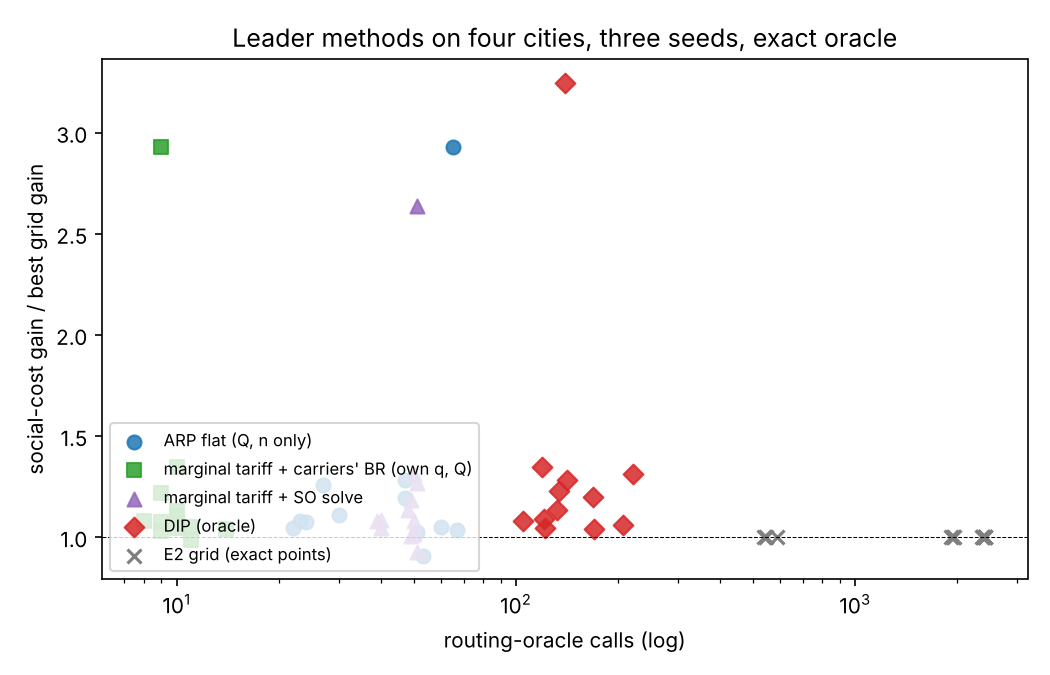
\includegraphics[width=0.65\textwidth]{arp_calls_vs_gain.png}
\caption{Leader methods on four cities and three seeds (exact oracle): gain relative to the best exact grid point against routing-oracle calls (log scale).}\label{fig:arp}
\end{figure}

%----------------------------------------------------------------------
\subsection{Robustness to the carriers' criterion}\label{sec:res-crit}

All game results above describe carriers who plan against the p-box worst-case route cost. To test how much this matters we recomputed the unpriced equilibrium, the price of anarchy, DIP and a coarse 16-point grid for carriers who plan with the sample-average cost of the same 30 days, with a Wasserstein ball with cross-validated radius, or with the theory radius, for all nine cities and \CritSeeds{} seeds. The SAA and Wasserstein carriers use a heuristic oracle without an optimality proof (equilibria verified against an independent fresh pool); the p-box reference uses price-and-branch; the coarse grid is easier to match than the 63-point grid. Table~\ref{tab:criterion} gives the three low-service cities.

\begin{table}[tbp]\centering\small
\caption{Game results under four carrier criteria, three seeds, mean. PoA with the true expected routing cost and with the carriers' own (model) cost. DIP gain as \% of $|$social cost$|$ under each cost. Best uniform per-delivery charge on the coarse grid as a fraction of the fee. Weighted DIP charge: $u_z/$fee weighted by deliveries.}\label{tab:criterion}
\adjustbox{max width=\linewidth}{\begin{tabular}{llrrrrrrrr}
\toprule
City & carriers' criterion & served share & PoA (true cost) & PoA (model cost) & DIP gain \%, true cost & DIP gain \%, model cost & best uniform charge / fee, true cost & same, model cost & DIP charge $u/$fee (weighted) \\
\midrule
New Delhi & p-box & 0.26 & 1.35 & 1.18 & 34.0 & 18.2 & -0.53 & -0.20 & -0.17 \\
New Delhi & SAA & 0.48 & 1.19 & 1.21 & 18.4 & 20.7 & -0.17 & -0.23 & -0.18 \\
New Delhi & Wass.\ CV & 0.46 & 1.19 & 1.20 & 18.5 & 19.4 & -0.20 & -0.20 & -0.18 \\
New Delhi & Wass.\ theory & 0.41 & 1.25 & 1.20 & 24.6 & 19.2 & -0.27 & -0.20 & -0.18 \\
Buenos Aires & p-box & 0.37 & 1.49 & 1.36 & 51.2 & 35.9 & -0.77 & -0.30 & -0.24 \\
Buenos Aires & SAA & 0.67 & 1.16 & 1.19 & 16.0 & 18.5 & -0.30 & -0.30 & -0.25 \\
Buenos Aires & Wass.\ CV & 0.58 & 1.27 & 1.23 & 26.6 & 23.5 & -0.37 & -0.23 & -0.25 \\
Buenos Aires & Wass.\ theory & 0.57 & 1.31 & 1.28 & 30.4 & 27.9 & -0.30 & -0.40 & -0.25 \\
London & p-box & 0.18 & 2.06 & 1.66 & 108 & 65.8 & -0.80 & -0.30 & -0.25 \\
London & SAA & 0.38 & 1.52 & 1.55 & 51.1 & 53.2 & -0.33 & -0.33 & -0.26 \\
London & Wass.\ CV & 0.32 & 1.69 & 1.65 & 68.0 & 63.8 & -0.47 & -0.40 & -0.26 \\
London & Wass.\ theory & 0.31 & 1.75 & 1.66 & 71.8 & 65.4 & -0.40 & -0.30 & -0.26 \\
\bottomrule
\end{tabular}
}
\end{table}

\paragraph{What is robust} Under all four criteria: the delivery charge alone achieves \CritDelShareMin--\CritDelShareMax{} of the best grid gain (\CritDelShareMinTh--\CritDelShareMaxTh{} for the theory radius); the congestion charge alone is small; the price of anarchy is at least 1.10 only in London, Buenos Aires and New Delhi (at most \CritPoaAboveOther{} elsewhere with SAA carriers); DIP's per-delivery charge follows $-0.375\,$fee$/n_z$ (slopes \CritSlopeMin--\CritSlopeMax, correlation at least \CritCorrAbsMin{} in absolute value); DIP matches the coarse-grid gain (ratio at least \CritDipGridMin) with \CritDipCallsShareSixThreeMin--\CritDipCallsShareSixThreeMax\% of the calls of a 63-point grid; the optimal charge is a subsidy in every city; and cities with complete service are unchanged.

\paragraph{What is not robust} The levels. With SAA carriers the unpriced served share roughly doubles (London \CritPbServedLondon{} to \CritSaaServedLondon, Buenos Aires \CritPbServedBuenosAires{} to \CritSaaServedBuenosAires, New Delhi \CritPbServedNewDelhi{} to \CritSaaServedNewDelhi) and the price of anarchy measured with the true cost falls (London \CritPbPoaTrueLondon{} to \CritSaaPoaTrueLondon, Buenos Aires \CritPbPoaTrueBuenosAires{} to \CritSaaPoaTrueBuenosAires, New Delhi \CritPbPoaTrueNewDelhi{} to \CritSaaPoaTrueNewDelhi). The ordering of the price of anarchy is not preserved: with SAA carriers it is \CritSaaBAND{} in Buenos Aires and New Delhi. The leader's gain under the true cost falls by half or more (London \CritPbDipTrueLondon\% to \CritSaaDipTrueLondon\%, Buenos Aires \CritPbDipTrueBuenosAires\% to \CritSaaDipTrueBuenosAires\%, New Delhi \CritPbDipTrueNewDelhi\% to \CritSaaDipTrueNewDelhi\%), and the best uniform charge for the true-cost objective shrinks by \CritChargeDropMin--\CritChargeDropMax\%, while DIP's zone charges themselves are almost unchanged. \emph{All levels of the price of anarchy, served share and gain in this paper describe carriers planning against a guaranteed upper bound; the orderings and the policy directions are robust, the levels are not.}

%----------------------------------------------------------------------
\subsection{Theory against data and verification}\label{sec:res-theory}\label{sec:res-verif}

The city games are of type D1, so the engine's profile is an exact pure equilibrium with E-threshold zero and Theorem~\ref{thm:main} holds trivially for it. To test the theorems non-trivially we computed the exact thresholds on mixed equilibria with belief weights equal to the realised aggregate (price-and-branch oracle; \SM{S5}, Table~S-theory). Non-trivial mixed equilibria were constructed from pairs of distinct pure equilibria; this succeeded in \ThGamesMixed{} of the \ThGamesTotal{} city-seed games, and \ThNoMixedCities{} have none because almost all demand is served. On all \ThProfiles{} tested profiles no statement of Theorem~\ref{thm:main} was violated (\ThViol{} violations). The bound is loose: the largest empirical threshold is \ThRatioMin--\ThRatioMax{} times the anchored bound (median \ThRatioMed). On these games $N\le6<d$, so the $(N-1)\bar\rho$ term is the smallest of the three in every case, and the $N$-free terms are not tested. Mixed equilibria were found only with two-plan supports. In all \ThGamCases{} (city, seed, $\delta$) cases the $\Gamma$-maximin surcharge equilibrium differs from the precise equilibrium, and the share of demand served drops by \ThGamDropLoMin--\ThGamDropLoMax{} at $\delta=0.1$ and by \ThGamDropHiMin--\ThGamDropHiMax{} at $\delta=1$. Under vehicle-count congestion the gadgets behave as proved: the tightness example has no pure equilibrium and threshold exactly $1/w$ (\ThPropOK{} weights), and the kernel construction reproduces the kernel sets for all four criteria on \ThKernOK{} digraphs. Among random bilinear D2 games with three players, \ThRandDtwo{} have no pure equilibrium, against \ThRandDone{} D1 controls; small routing-integrated D2 games always had a pure equilibrium (\ThTiny{}), and on the city games of Cairo, Mumbai and Paris with a vehicle-count externality scaled by \ThCityScales{}, all \ThCityRuns{} best-response runs converged. Non-existence required adversarial plan menus.

On \TinyN{} tiny games solved by exhaustive enumeration, the engine's profile is a pure equilibrium in every case and reaches the global potential minimum in \TinyZMCglobal{} of \TinyN{} (best response \TinyBRglobal, Frank--Wolfe with rounding \TinyFWglobal, column generation \TinyCGglobal). At city scale every base equilibrium, every verified grid best point (\VerBestN{} city-seeds) and every equilibrium of the price-of-anarchy experiment has regret at most \ExRegretFreshMax{} USD against an independent fresh exact oracle. Because some oracle calls were not proven optimal, the guaranteed regret bound is nonzero for \ExBoundN{} profiles, at most \ExBoundMax{} USD. These checks rely on the same branch-and-price method as the oracle; the pricer was checked against enumeration (Section~\ref{sec:res-brl}).

%======================================================================
\section{Implications and limitations}\label{sec:discussion}\label{sec:implications}\label{sec:limits}

The model is stylised and several parameters are weak (Section~\ref{sec:data}), so the effects below are qualitative: they indicate what to test with local data, not what to do in any particular city.

\paragraph{Where pricing matters} In the model, the efficiency loss from competition is concentrated where service is incomplete. Where carriers already serve almost all demand (Cairo, Moscow, New York, Paris, Berlin), the price of anarchy is close to one and charges change little; kerb space and background traffic are the more relevant levers there. Where service is partial, the instrument with the largest effect is a per-delivery subsidy, which in every material case was the best flat charge. A congestion charge on vehicle-hours alone gains much less but not nothing. The gains depend strongly on the sampled slice and the ordering of the cities by price of anarchy holds in \TenPoaOrderAll{} of \TenPoaOrderN{} seeds only, so the direction is better supported than the size. A subsidy has a fiscal cost that the welfare criterion with transfers does not count, access stays unequal in the low-service cities, and an objective that counts delay to other road users can reverse the recommendation.

\paragraph{How a city could compute charges} A city does not need to search a grid. With the carriers' routing oracle, DIP gives zone charges at \TenDipCallsNewDelhi--\TenDipCallsLondon\% of a 63-point grid's calls, with a readable structure: a subsidy of roughly 37.5\% of the fee divided by the number of carriers in the zone, corrected for congestion. Without the oracle, ARP needs only the zone totals after each posted charge, and the marginal tariff needs billing on own deliveries and the zone total; the flat rule can cycle or settle in a worse local optimum and the tariff stops at a unilateral social optimum, so a pilot with a few posted charges is a cheap check. Because all levels describe carriers who plan against a guaranteed upper bound, a city should calibrate the level of any charge on observed carrier behaviour and treat our magnitudes as indicative. A carrier with enough data to estimate the law should weigh that the p-box criterion costs expected cost (\AmbRegMin--\AmbRegMax\% at up to 60 training days) in exchange for tail protection and a bound.

\paragraph{Smart-city relevance} The study is an offline simulation on open data. It contains no machine learning, digital twin, real-time control or experiment with decision makers. The instances are built from open data and public parameters, and each carrier's uncertainty set is built from 30 observed days of travel times. DIP and the marginal tariff let the city compute zone charges that make a chosen social outcome stable, and ARP needs only zone totals, the information that a reporting or billing arrangement between city and carriers could supply; ARP's loop of posting a charge, observing the totals and updating is the form a pilot would take. The charges are simple to state, but the model does not represent fairness across carriers or neighbourhoods, and whether the methods work with a human in the loop or on live data is not tested here.

\paragraph{Limitations}
\begin{itemize}[leftmargin=*,itemsep=0pt]
\item \emph{Model.} Lots are all-or-nothing (S1), so part of the measured inefficiency may be an artifact of indivisibility. Congestion is linear and, within a zone, proportional to deliveries (S3, S4). Demand is sampled, market shares are equal in seven cities, and the congestion coupling is scaled by a slice multiplicity. Most operating parameters are country-level or rough; delivery fee, drops per vehicle and the number of carriers move welfare by tens of per cent over their plausible ranges (\SM{S4}), and the sign of the best per-delivery instrument depends on the fee-to-cost ratio.
\item \emph{Exactness and coverage.} \ExUnproven{} of \ExCalls{} oracle calls were not proven optimal; for \ExBoundN{} profiles the guaranteed regret bound is positive (at most \ExBoundMax{} USD). The grid is exact in full only for \ExEtwoFullCities, so the grid's gains in the other six cities are lower bounds; the engine comparison, ZMC checks, theory tests and tiny-game verification use price-and-branch. Branch-and-price was tested only on instances with 22 customer zones.
\item \emph{Carriers' criterion and BRL.} The robustness study used a heuristic oracle for sample-average and Wasserstein carriers, a coarse 16-point grid and three seeds. The out-of-sample comparison of criteria uses one slice per city and a heuristic planner validated against branch-and-price in nine instances. BRL does not beat sample-average or Wasserstein plans on held-out cost, was not compared with resource-extension-function dominance, and was benchmarked on public instances only by an emulation.
\item \emph{Leader methods.} DIP is no better than its social target, its selection is optimistic, its closed forms need D1 and one hours-per-delivery ratio, and the subsidies it requires under strong ambiguity aversion are unrealistic. ARP was run on four cities, can cycle, can settle in a worse local optimum, and has no guarantee for the pure game unless its fixed point is reached. Neither method has a worst-equilibrium guarantee.
\item \emph{Theory.} The credal results assume affine coupling. The absorption tests rely on two-plan mixed equilibria; the full rounding algorithm was not run on real data; D2 was tested only with a calibration introduced for the test. The Lean formalisation covers only the finite and algebraic cores listed in \SM{S12}.
\item \emph{Evidence and novelty checks.} Seeds vary the sampled slice, not the calibration inputs. Ten seeds exist only for \TenFullCities. Price-of-anarchy values come from at most six equilibria per city and seed. Novelty searches were web and index searches, partly at the level of abstracts, and a Scopus and Web of Science search has not been done. The closest neighbours \citep{GhosalHoWiesemann2024,Masiha2026,Feik2026,Beauchene2016,LiuMaMa2026,Irnich2008} were read in full text (the first in its October 2021 preprint version, Beauch\^ene's paper as main text and Liu--Ma--Ma as pp.\ 1--13). \citet{Lanzetti2025}, the trial-and-error toll papers, the budgeted-uncertainty pricing papers, the function-label papers \citep{Dabia2013,Ioachim1998} and the other neighbours were read in part or at abstract level.
\end{itemize}
Open questions include the complexity of finding a pure E-admissible equilibrium above the guaranteed width (we conjecture PPAD-hardness), smoothness constants for the Cournot--congestion game, an absorption result for nonaffine congestion, worst-equilibrium guarantees for the leader, and carrier-level data that would replace our proxies.

%======================================================================
\section{Conclusion}\label{sec:conclusion}

A city that prices competing delivery carriers faces NP-hard best responses under probability-box travel times, a congestion game among the carriers and a bilevel search over charges. We gave an algorithm for each layer and tested them on nine metropolitan areas.

\emph{Carriers' routing.} BRL prices routes exactly under the dependence-robust criterion and, with branch-and-price, proved optimal robust plans on all nine metro instances with 22 customer zones. Its window rule keeps fewer labels than weaker rules, but the gain shrinks on real data, the plans do not beat sample-average plans out of sample, and exact solution is shown only up to 22 customer zones in all nine cities and 30 to 40 customers in London and New York.

\emph{City charges.} DIP made its target an exact equilibrium in every run and reached \TenDipGridBuenosAires--\TenDipGridNewDelhi{} times the best grid point's gain with \TenDipCallsNewDelhi--\TenDipCallsLondon\% of its calls in the three cities with ten seeds, partly because its charges are zone-specific; against the social optimum the grid reaches \TenSoGridNewDelhi--\TenSoGridBuenosAires{} and DIP \TenSoDipNewDelhi--\TenSoDipLondon. ARP, which sees only zone totals, reached \TenSoArpNewDelhi--\TenSoArpBuenosAires{} of the social optimum's gain and contracts at a rate independent of instance size in the convexified game; in the pure game it can cycle or settle in a worse local optimum.

\emph{Theory.} Pure equilibria exist under exposure-based congestion and deciding existence is strongly NP-complete under vehicle-count congestion. The credal absorption width has an $(N-1)$ term that is attained at $N=2$ and binds on the city instances, and the theorem is close to earlier work on approximate equilibria.

\emph{Cities.} The price of anarchy is near one where service is complete and larger where it is partial, with a wide spread over seeds and an ordering that holds in \TenPoaOrderAll{} of \TenPoaOrderN{} seeds. A per-delivery subsidy captures most of the grid leader's gain; a congestion charge alone captures much less but sometimes more than 1.7\%. These levels describe carriers who plan against a guaranteed upper bound: with sample-average carriers service roughly doubles and the leader's gain falls by half or more, while orderings and policy directions persist. The findings come from stylised slices with weak parameters, and the novelty of each component is limited as stated in Section~\ref{sec:intro}. The observation-only methods, ARP and the marginal tariff, are the natural candidates for a pilot with real data.

\section*{Data and code availability}
Code, processed data, parameter sources, result files, figures and the scripts that generate the tables and numbers of this paper are available at \url{https://github.com/vinhqdang/Competing-Carriers-under-Uncertainty}. Raw OpenStreetMap extracts are distributed under the Open Database License; GHS-POP is distributed by the European Commission Joint Research Centre.

\section*{Declaration of competing interest}
The author declares no competing financial interests or personal relationships that could have appeared to influence the work reported in this paper.

\section*{Funding}
This research received no specific grant from any funding agency in the public, commercial or not-for-profit sectors.

\bibliographystyle{elsarticle-num-names}
\bibliography{references}

\end{document}
